\documentclass[a4paper]{beamer}%handout


\usepackage{listings}
\usepackage{color}
 
\definecolor{codegreen}{rgb}{0,0.6,0}
\definecolor{codegray}{rgb}{0.5,0.5,0.5}
\definecolor{codepurple}{rgb}{0.58,0,0.82}
\definecolor{backcolour}{rgb}{0.95,0.95,0.92}


%% Add Matlab code
\usepackage{mcode}
%% Add Matlab code end


%% Add watermarks
%\usepackage{draftwatermark}
%% Add watermarks end
\usepackage[utf8]{inputenc}
\usepackage{multicol}
\usepackage{url}
\usepackage{hyperref}
\hypersetup{
	colorlinks=true,
	linkcolor=cyan,          % color of internal links (change box color with linkbordercolor)
    citecolor=green,        % color of links to bibliography
    filecolor=magenta,      % color of file links
    urlcolor=cyan           % color of external links
	}

\graphicspath{{img/}}

\mode<presentation> {

%\usetheme{default}%yes % use %\frametitle in all slides recommended
%\usetheme{AnnArbor}%no
%\usetheme{Antibes} %yes %favorite
%\usetheme{Bergen} %no
%\usetheme{Berkeley} %no
%\usetheme{Berlin} %no
%\usetheme{Boadilla} %yes % good use of paper space
%\usetheme{CambridgeUS} %yes %favorite %use %\frametitle recommended
%\usetheme{Copenhagen}%yes%noframetitle
%\usetheme{Darmstadt}%no
%\usetheme{Dresden}
%\usetheme{Frankfurt}
%\usetheme{Goettingen}
%\usetheme{Hannover}
%\usetheme{Ilmenau}%no
%\usetheme{JuanLesPins}
%\usetheme{Luebeck}
%\usetheme{Madrid}
%\usetheme{Malmoe}
%\usetheme{Marburg}
%\usetheme{Montpellier}
%\usetheme{PaloAlto}
%\usetheme{Pittsburgh}%no
%\usetheme{Rochester}%no
%\usetheme{Singapore}%yees
%\usetheme{Szeged}%no
%\usetheme{Warsaw}%no

% As well as themes, the Beamer class has a number of color themes
% for any slide theme. Uncomment each of these in turn to see how it
% changes the colors of your current slide theme.

%\usecolortheme{albatross}
%\usecolortheme{beaver}
%\usecolortheme{beetle}
%\usecolortheme{crane}
\usecolortheme{dolphin}
%\usecolortheme{dove}
%\usecolortheme{fly}
%\usecolortheme{lily}
%\usecolortheme{orchid}
%\usecolortheme{rose}
%\usecolortheme{seagull}
%\usecolortheme{seahorse}
%\usecolortheme{whale}
%\usecolortheme{wolverine}

\setbeamertemplate{footline} % To remove the footer line in all slides uncomment this line
%\setbeamertemplate{footline}[page number] % To replace the footer line in all slides with a simple slide count uncomment this line

\setbeamertemplate{navigation symbols}{} % To remove the navigation symbols from the bottom of all slides uncomment this line
}

%----------------------------------------------------------------------------------------
%	NEW COMMANDS
%----------------------------------------------------------------------------------------

\newcommand{\Conv}{\mathop{\scalebox{1.5}{\raisebox{-0.2ex}{$\ast$}}}}%
%\linespread{1.3}

%----------------------------------------------------------------------------------------
%	TITLE PAGE
%----------------------------------------------------------------------------------------

\title[Introduction]{Digital Image Processing} % The short title appears at the bottom of every slide, the full title is only on the title page

\author{Prof. Tiago Vieira} % Your name
\institute[UFAL] % Your institution as it will appear on the bottom of every slide, may be shorthand to save space
{
Universidade Federal de Alagoas \\ % Your institution for the title page
\medskip
\textit{tvieira@ic.ufal.br} % Your email address
}
\date{\today} % Date, can be changed to a custom date


%----------------------------------------------------------------------------------------
%	TITLE PAGE
%----------------------------------------------------------------------------------------

\title[Morphology]{Digital Image Processing} % The short title appears at the bottom of every slide, the full title is only on the title page

\author{Prof. Tiago Vieira, PhD} % Your name
\institute[UFAL] % Your institution as it will appear on the bottom of every slide, may be shorthand to save space
{
Universidade Federal de Alagoas \\ % Your institution for the title page
\medskip
\textit{tvieira@ic.ufal.br} % Your email address
}
\date{\today} % Date, can be changed to a custom date

%------------------------------------------------

\begin{document}

%------------------------------------------------

\begin{frame}
\titlepage % Print the title page as the first slide
\end{frame}

%------------------------------------------------

\begin{frame}
\frametitle{Contents}
    \setcounter{tocdepth}{1}
    \begin{columns}[t]
        \begin{column}{.5\textwidth}
            \tableofcontents[sections={1-4}]
        \end{column}
        \begin{column}{.5\textwidth}
            \tableofcontents[sections={5-8}]
        \end{column}
    \end{columns}
\end{frame}

%----------------------------------------------------------------------------------------
%	PRESENTATION SLIDES
%----------------------------------------------------------------------------------------

\section{Introduction}

\subsection{Morphology}

\begin{frame}
\frametitle{Introduction}
\begin{itemize}
\item Morphology = study of forms.
\item Useful for describing image components:
\begin{itemize}
\item Boundaries.
\item Skeletons.
\item Convex hull.
\end{itemize}
\item Also useful for pre- and post-processing:
\begin{itemize}
\item Filtering.
\item Thinning.
\item Pruning.
\end{itemize}
\end{itemize}
\end{frame}

\subsection{Set theory}

\begin{frame}
\frametitle{Set theory}
Set theory is fundamental to understand morphology.
\begin{itemize}
\item Sets represent objects in an image.
\item The set of all white pixels is a complete representation of this image.
\item In binary images:
\begin{itemize}
\item sets are members of $\mathcal{Z}^{2}$ (bi-dimensional space of integers).
\item each element $z_{i}$ is a bi-dimensional vector of coordinates $(x_{i}, y_{i})$.
\end{itemize}
\item In grayscale images:
\begin{itemize}
\item Set components are in $\mathcal{Z}^{3}$.
\end{itemize}
\end{itemize}
\end{frame}

\begin{frame}
%\frametitle{Set theory}
Consider $A$ a set in $\mathcal{Z}^{2}$.\\
If $w_{i} = (x_{i}, y_{i})$ is an element of $A$, then $w \in A$.\\
If $w$ is not an element of $A$, then $w \notin A$.\\
Also:\\
\begin{tabular}{|l|l|}
\hline 
Empty set & $\emptyset$ \\ 
$A$ subset of $B$ & $A \subseteq B$ \\ 
Union of $A$ and $B$ & $A \cup B$ \\ 
Intersection between $A$ and $B$ & $A \cap B$ \\
Disjoint sets & $A \cap B = \emptyset$ \\ 
Set specification & $B = \{ w | \text{condition}$ \} \\ 
\hline
\end{tabular} 
\end{frame}

\begin{frame}
%\frametitle{Set theory}
Also:\\
\begin{tabular}{|l|l|}
\hline 
Complement of $A$ & $A^{c} = \{ w | w \notin A \}$\\
Difference between $A$ and $B$ & $A - B = \{ w | w \in A, w \notin B \}$ \\
Reflection of $B$ & $\hat{B} = \{ w | w = -b, b \in B \}$ \\
Translation of $A$ by $z = ( x, y )$ & $\left ( A \right )_{z} = \{ c | c = a + z, a \in A \}$ \\
\hline
\end{tabular} 
\end{frame}

\begin{frame}
%\frametitle{Set theory}
\begin{figure}[!h]
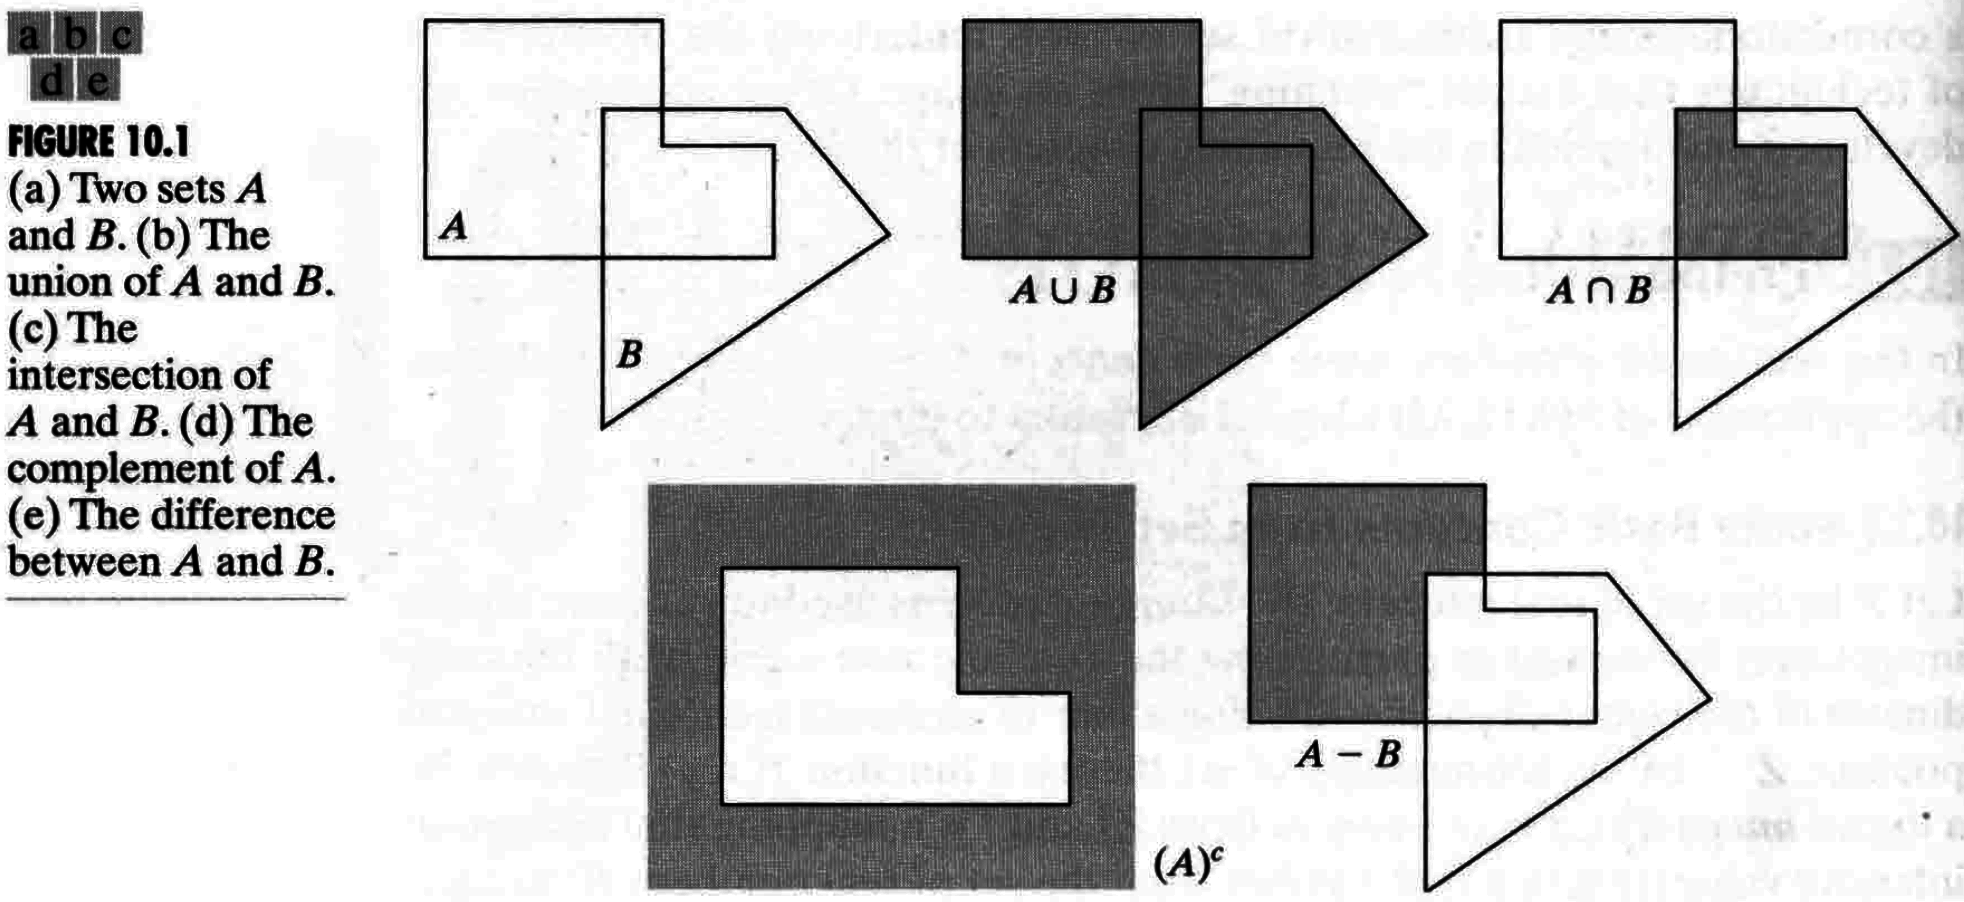
\includegraphics[width=.8\textwidth]{fig-10-1}
\end{figure}
\begin{figure}[!h]
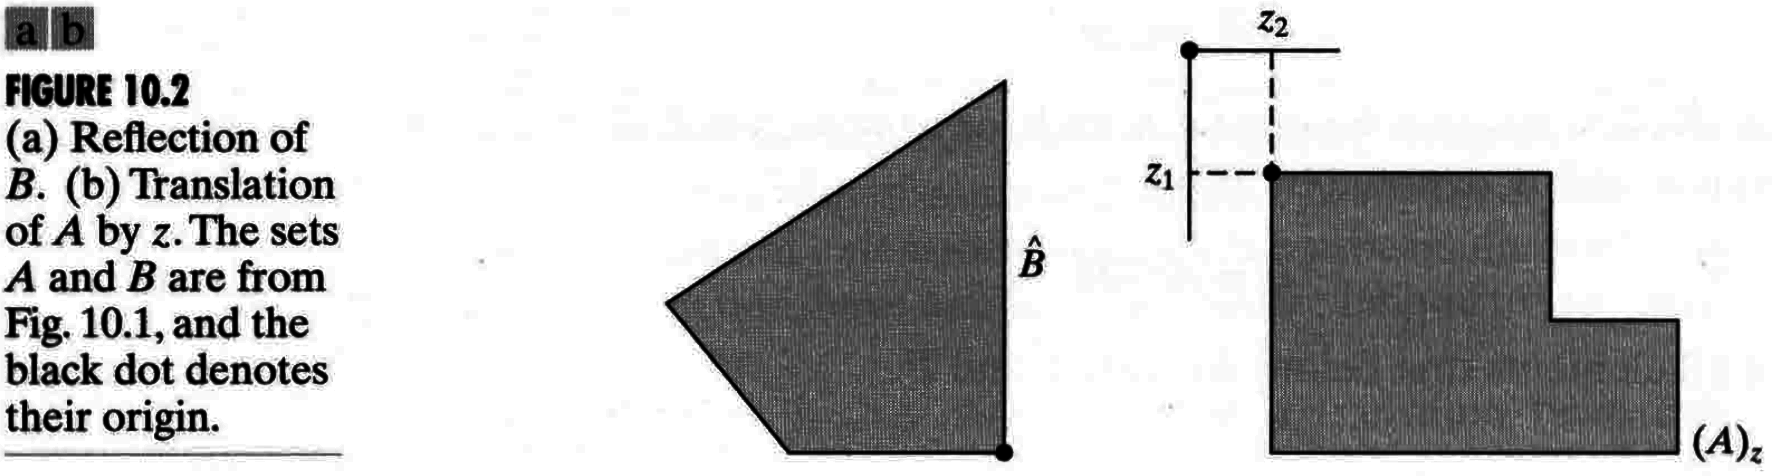
\includegraphics[width=.8\textwidth]{fig-10-2}
\end{figure}
\end{frame}

\subsection{Logical operators}

\begin{frame}
\frametitle{Logical operators}
\begin{figure}[!h]
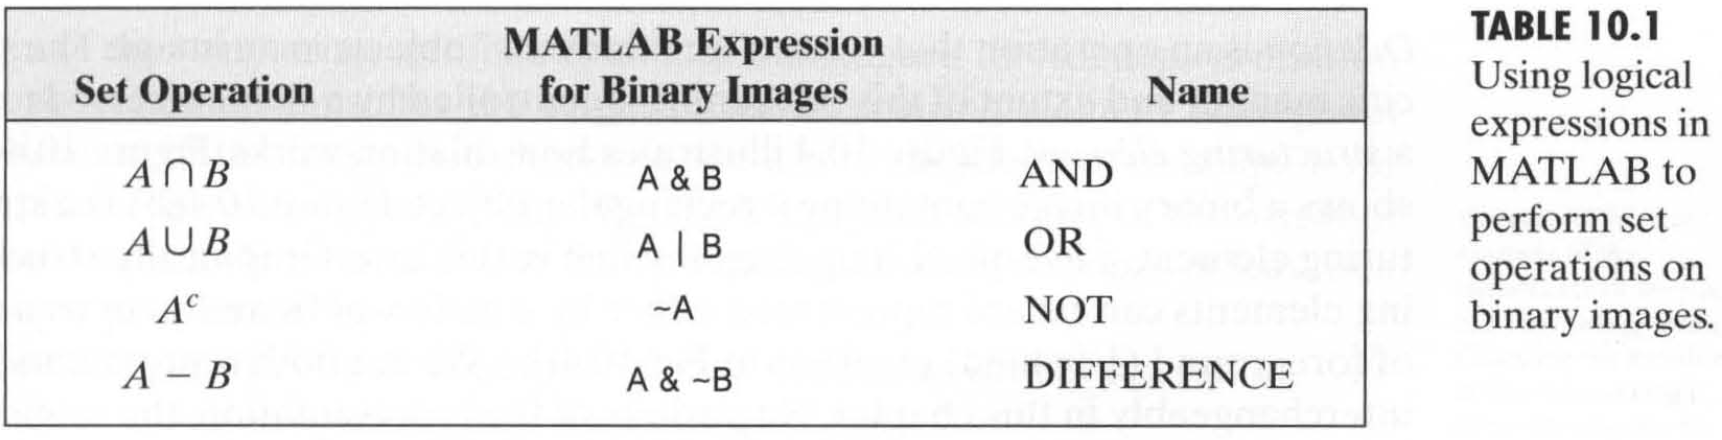
\includegraphics[width=\textwidth]{table-10-1.png}
\end{figure}
\begin{figure}[!h]
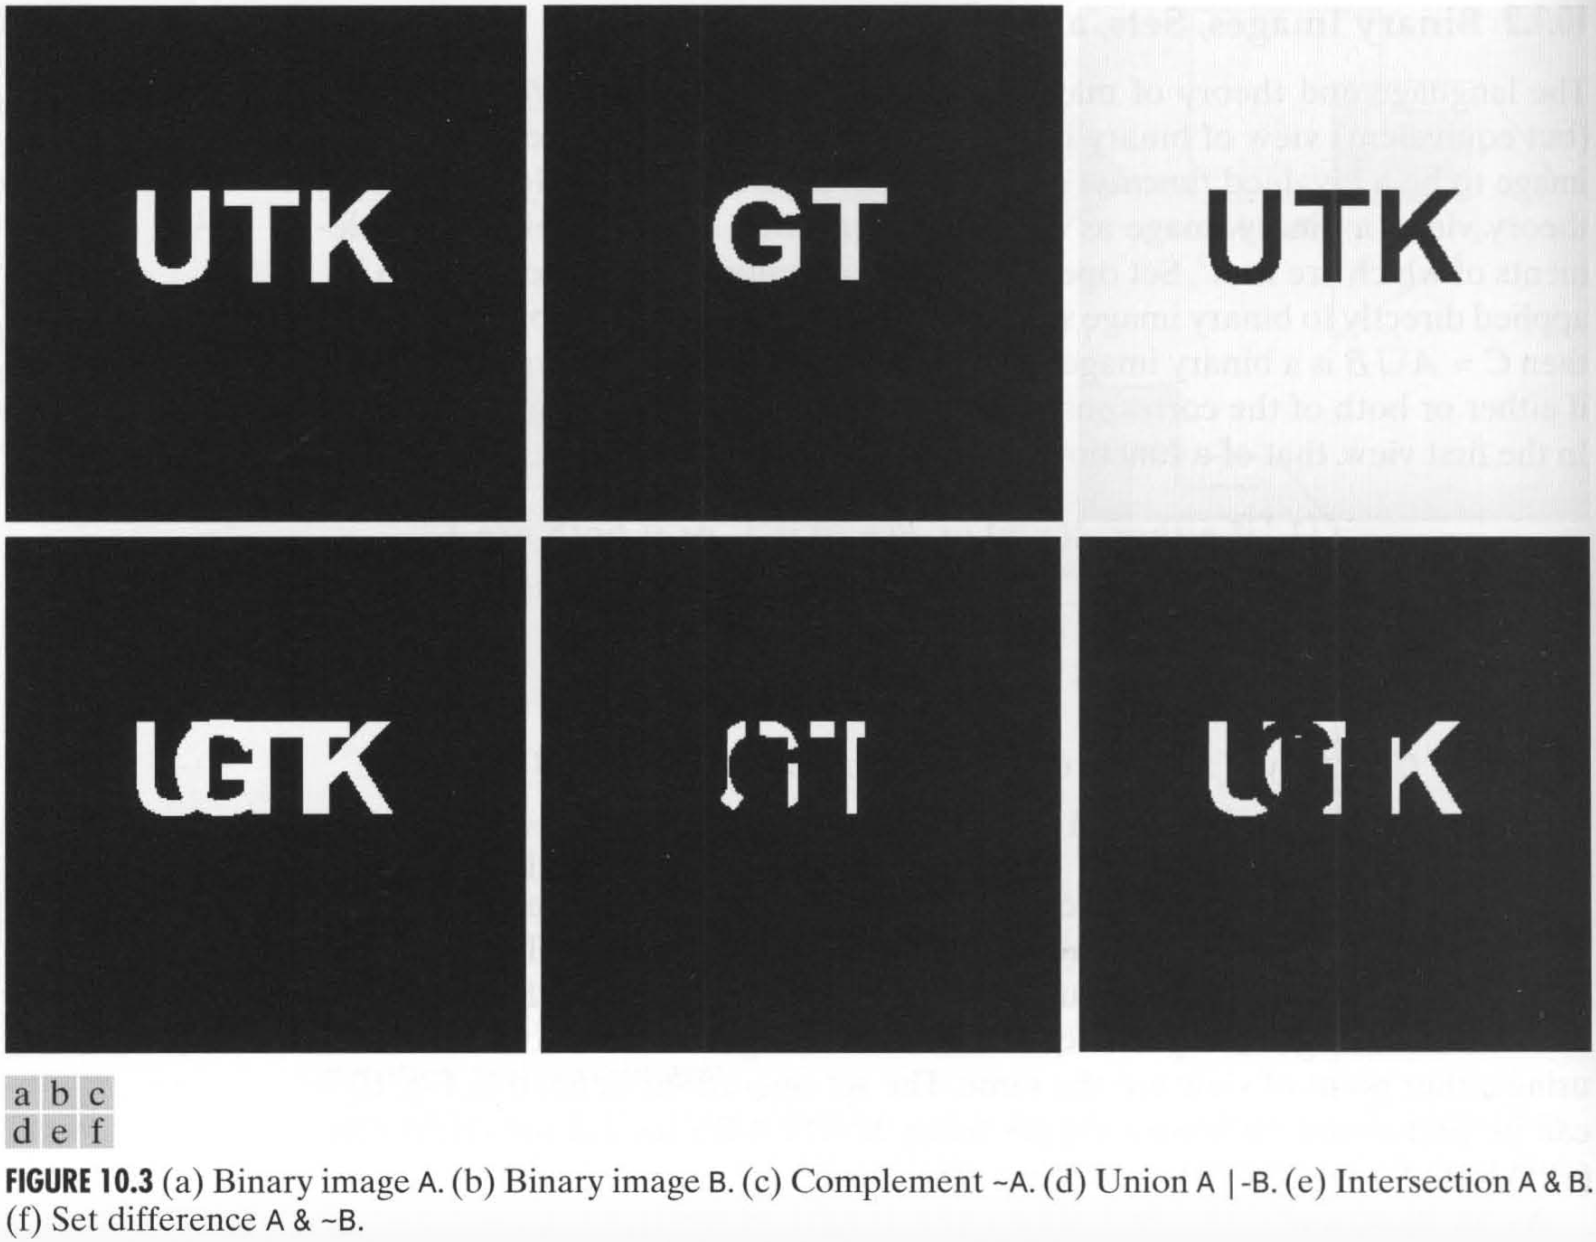
\includegraphics[width=.4\textwidth]{fig-10-3.png}
\end{figure}
\end{frame}

\section{Dilation and erosion}

\subsection{Dilation}

\begin{frame}
\frametitle{Dilation}
\begin{columns}
\begin{column}{.5\textwidth}
\begin{block}{Definition}
$A \oplus B = \left \{ z | \left ( \hat{B} \right )_{z} \cap A \neq  \emptyset \right \}$\\
$A\oplus B = \left \{ z | [ (\hat{B})_{z} \cap A ] \subseteq A \right \}$
\end{block}
\begin{itemize}
\item Reflexion of $B$ followed by a translation of $z$.
\item Result contains all shifts $z$ st. there is at least one intersection between $A$ and $B$.
\end{itemize}
\end{column}
\begin{column}{.5\textwidth}
\begin{itemize}
\item $B$ is the \textit{Structuring Element} (SE).
\end{itemize}
Example:
\begin{figure}[!h]
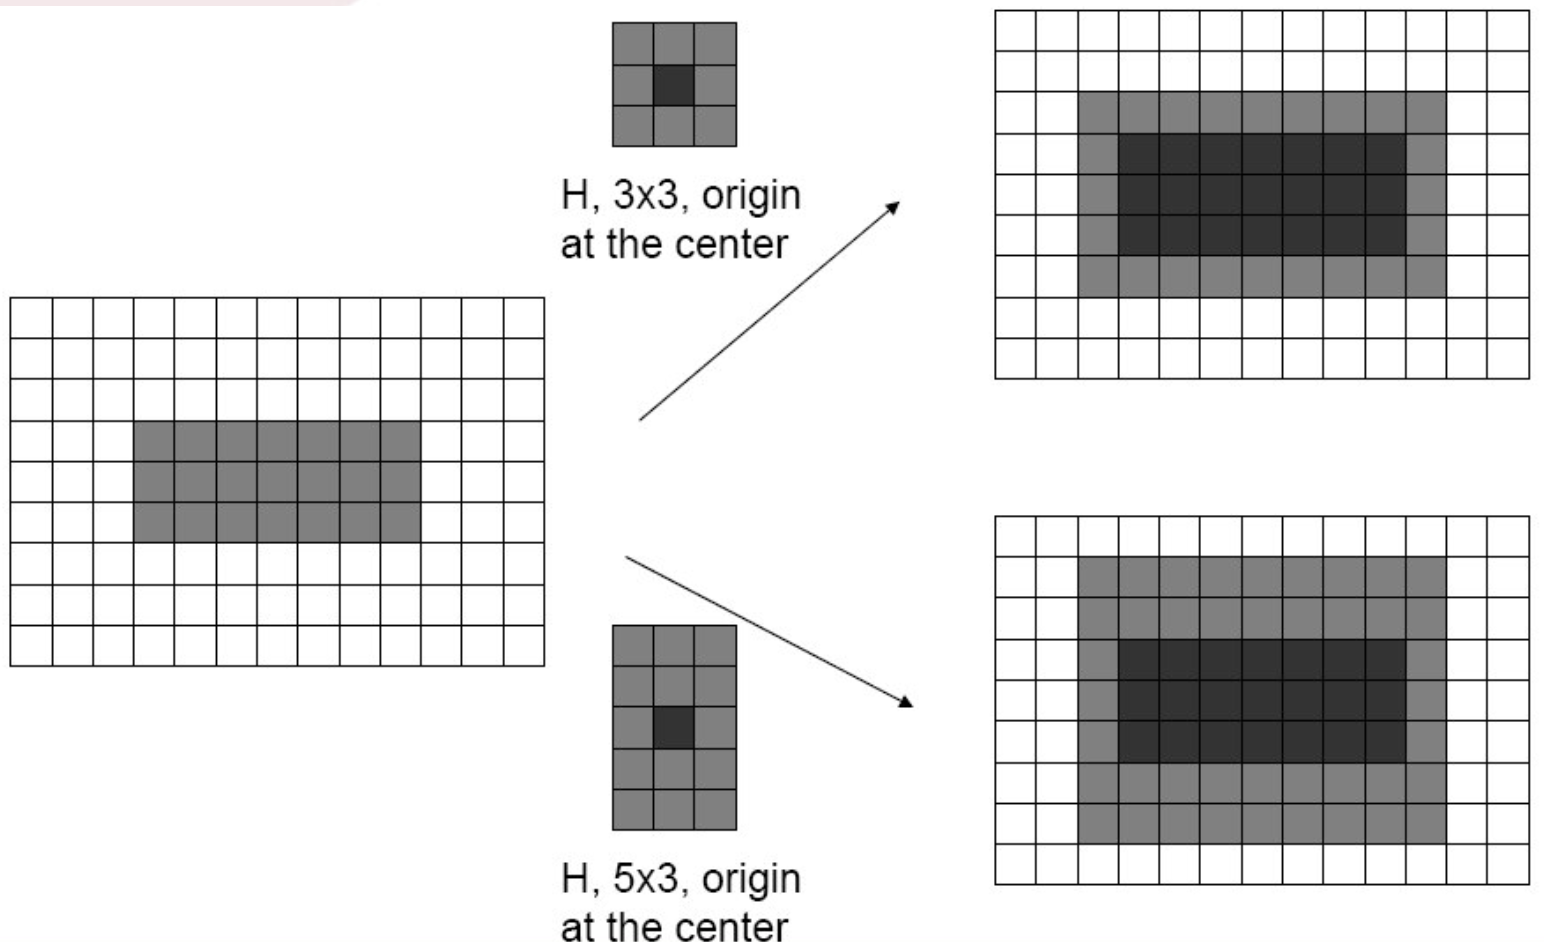
\includegraphics[width=\textwidth]{dilation-ex-1}
\end{figure}
\end{column}
\end{columns}
\end{frame}

\begin{frame}
\begin{columns}
\begin{column}{.5\textwidth}
\begin{block}{Properties of dilation}
\begin{itemize}
\item Associativity $A \oplus \left ( B \oplus C \right ) = \left ( A \oplus B \right ) \oplus C$.\\
\item Commutativity $A \oplus B = B \oplus A$.
\end{itemize}
\end{block}
\end{column}
\begin{column}{.5\textwidth}
Another example:
\begin{figure}[!h]
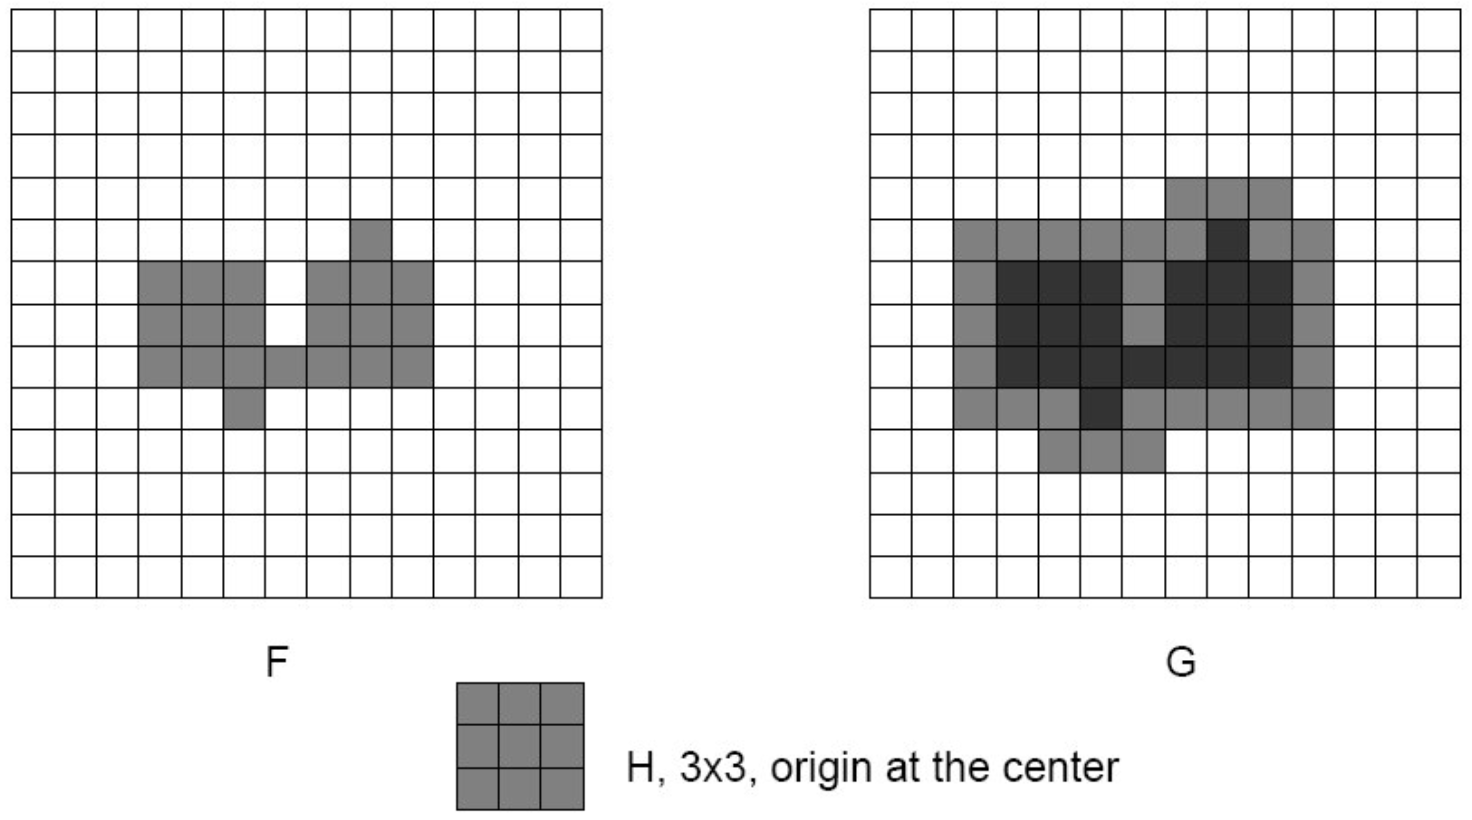
\includegraphics[width=\textwidth]{dilation-ex-2}
\end{figure}
\end{column}
\end{columns}
\end{frame}

\begin{frame}
Application: Gap filling.
\begin{figure}[!h]
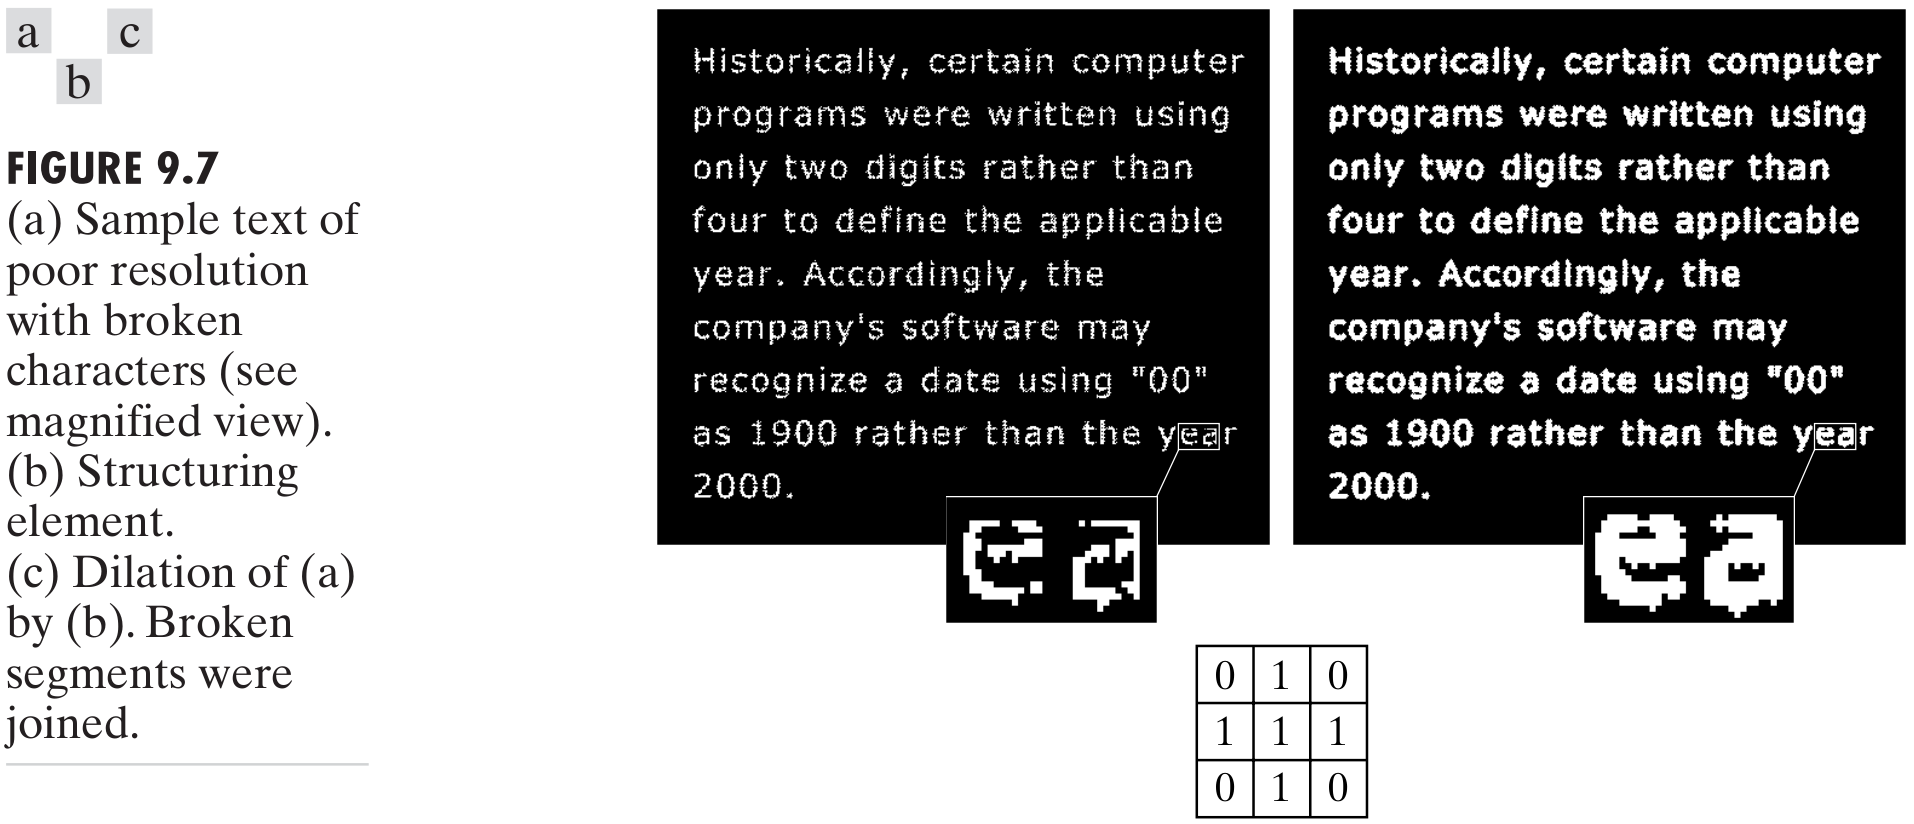
\includegraphics[width=\textwidth]{fig-9-7.png}
\end{figure}
\end{frame}

%\begin{frame}
%\begin{lstlisting}[language=Python, caption=Python example]
%img = cv2.imread(os.path.join(folder, 'text.tif'), cv2.IMREAD_GRAYSCALE)
%kernel = np.zeros((3, 3), dtype='uint8')
%kernel[:, 1] = 1
%kernel[1, :] = 1
%print(kernel)
%
%img2 = cv2.dilate(img, kernel, iterations=1)
%
%plt.subplot(121), plt.imshow(img, cmap='gray')
%plt.subplot(122), plt.imshow(img2, cmap='gray')
%plt.show()
%\end{lstlisting}
%\end{frame}

\subsection{Erosion}

\begin{frame}
\frametitle{Erosion}
\begin{columns}
\begin{column}{.5\textwidth}
\begin{block}{Definition}
$A \ominus B = \left \{ z | \left ( B \right )_{z} \subseteq A \right \}$\\
$A \ominus B = \left \{ z | \left (B\right )_{z}  \cap A^{c} = \emptyset \right \}$
\end{block}
\begin{itemize}
\item Result contains all shifts $z$ st. $B$ lies inside $A$.
\end{itemize}
\end{column}
\begin{column}{.5\textwidth}
Example:
\begin{figure}[!h]
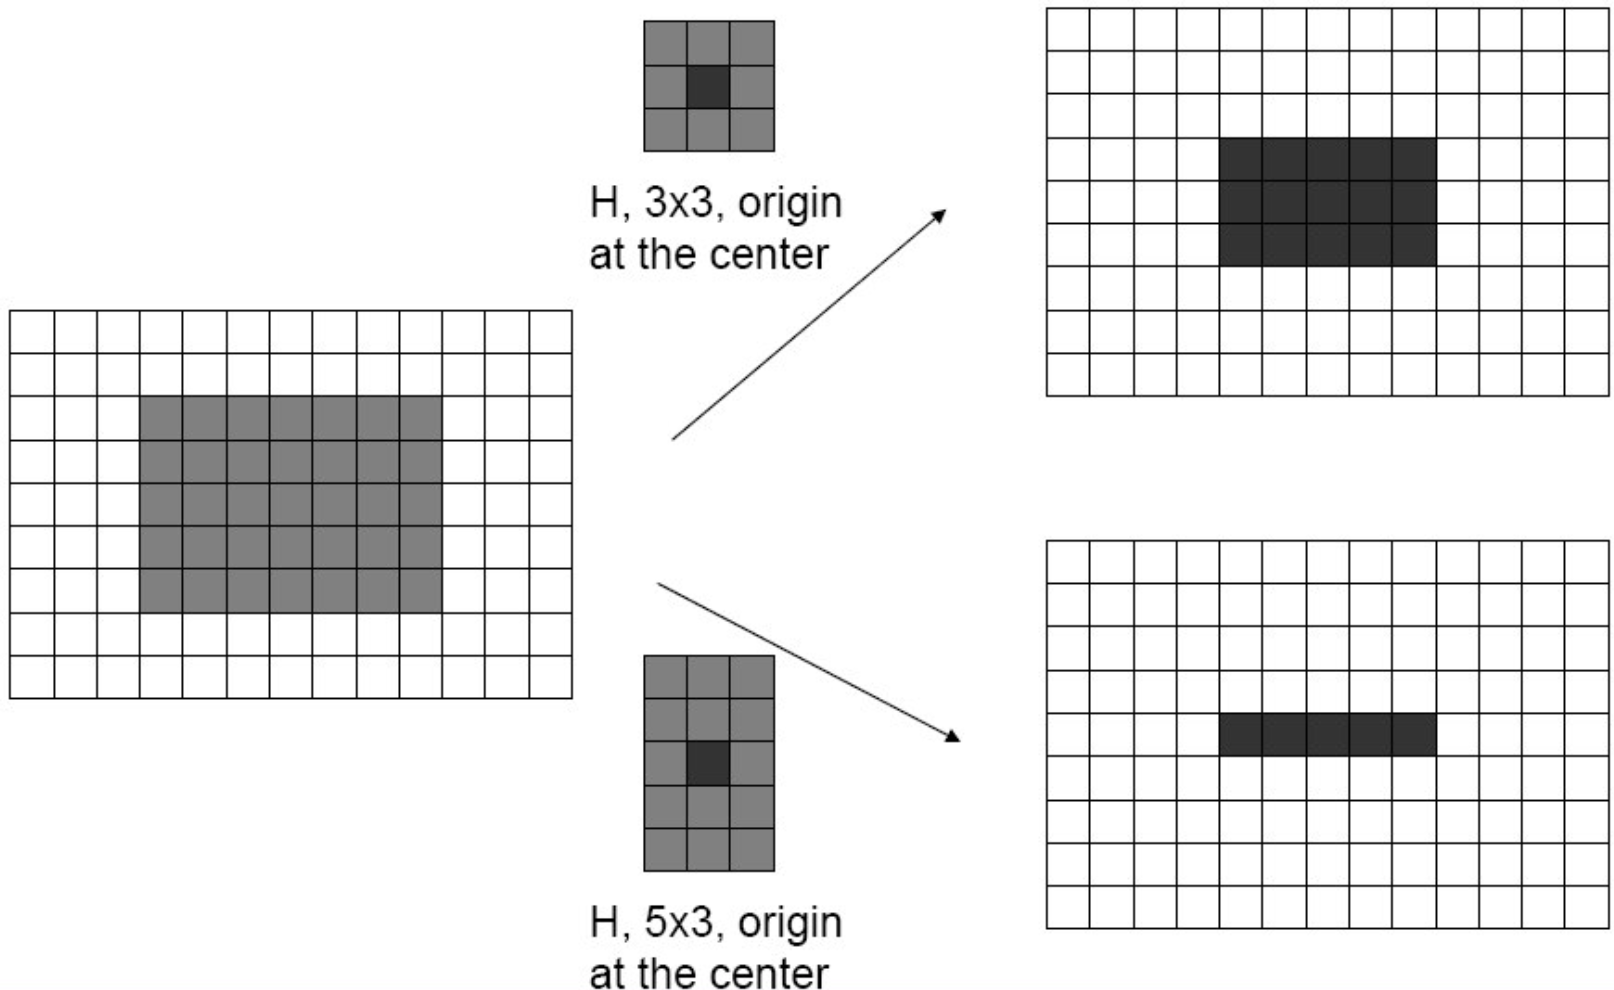
\includegraphics[width=\textwidth]{erosion-ex-1}
\end{figure}
\end{column}
\end{columns}
\end{frame}

\begin{frame}
\begin{columns}
\begin{column}{.5\textwidth}
\begin{block}{Properties of erosion}
\begin{itemize}
\item It is NOT commutative:
\[A \ominus B \neq B \ominus A.\]
\item It is NOT associative, but:
\[(A \ominus B)\ominus C \neq A \ominus (B \ominus C).\]
\end{itemize}
\end{block}
\end{column}
\begin{column}{.5\textwidth}
Another example:
\begin{figure}[!h]
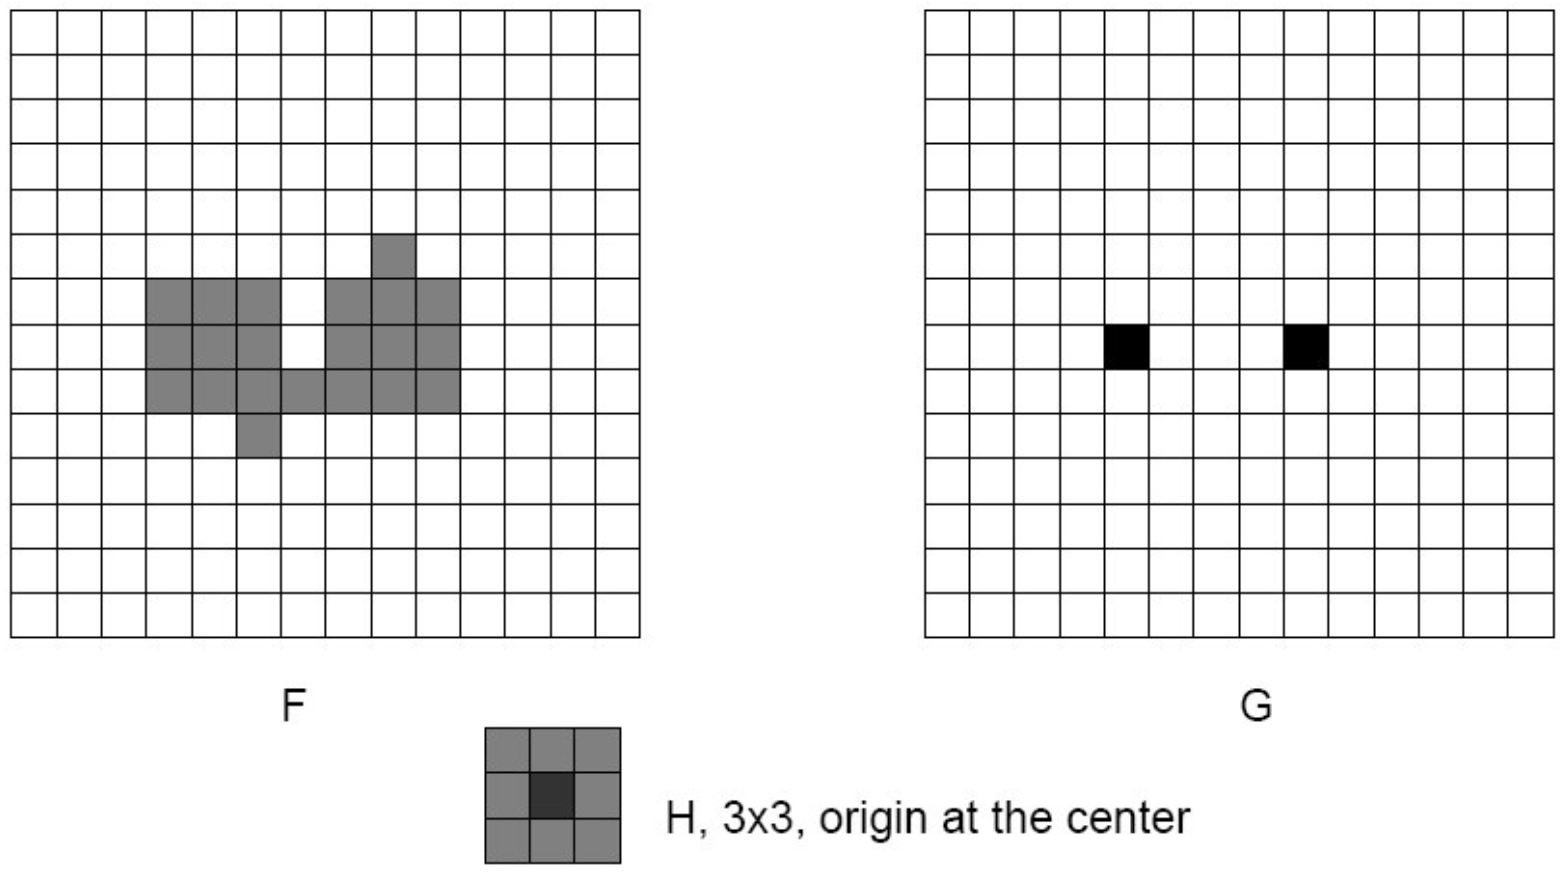
\includegraphics[width=\textwidth]{erosion-ex-2}
\end{figure}
\end{column}
\end{columns}
\end{frame}

\begin{frame}
Application: Removing image components.
\begin{figure}[!h]
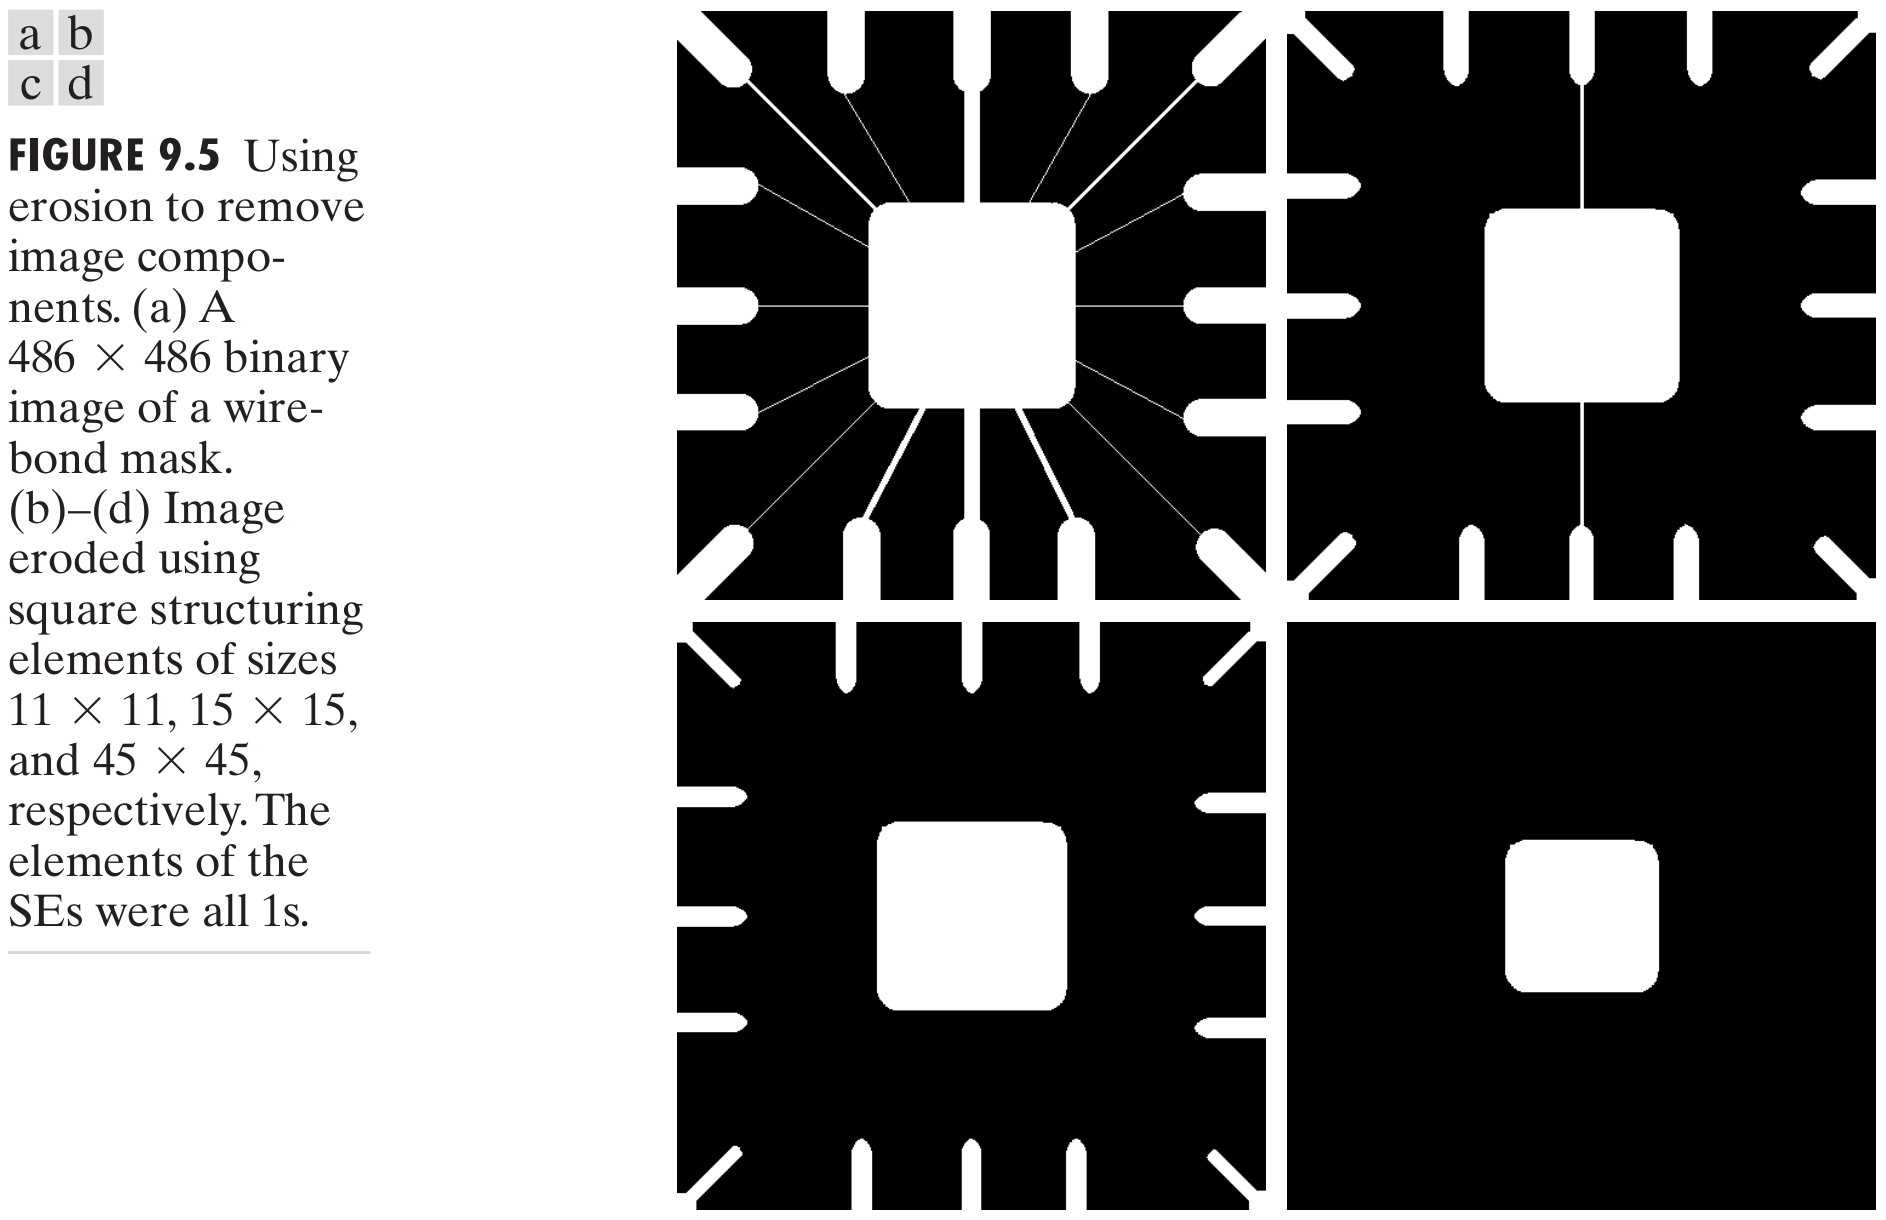
\includegraphics[width=.8\textwidth]{fig-9-5}
\end{figure}
\end{frame}

\subsection{Dilation and erosion}

\begin{frame}
\frametitle{Dilation and erosion}
\begin{block}{Duality}
Erosion and Dilation are duals of each other wrt. set complementation and reflection:
\begin{itemize}
\item $\left (A \oplus B\right )^{c} = A^{c} \ominus \hat{B}$.
\item $\left ( A \ominus B \right )^{c} = A^{c} \oplus \hat{B}$.
\end{itemize}
\end{block}
\end{frame}

\section{Opening and closing}

\subsection{Opening}

\begin{frame}
\frametitle{Opening}
\begin{columns}
\begin{column}{.3\textwidth}
\begin{figure}
\centering
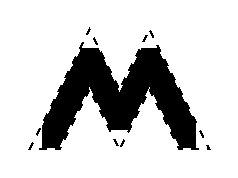
\includegraphics[width=\textwidth]{openb.png}
\end{figure}
\end{column}
\begin{column}{.7\textwidth}
\begin{itemize}
\item Erosion followed by a dilation:
\[A \circ B = \left ( A \ominus B  \right ) \oplus B\]
\item Effect similar to erosion (tends to remove background).
\item Less destructive than erosion.
\item Determined by a structuring element.
\end{itemize}
\end{column}
\end{columns}
\end{frame}

\begin{frame}
\begin{columns}
\begin{column}{.3\textwidth}
\begin{figure}
\centering
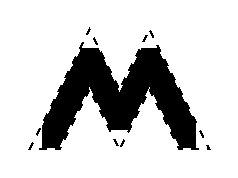
\includegraphics[width=\textwidth]{openb.png}
\end{figure}
\end{column}
\begin{column}{.7\textwidth}
Tends to:
\begin{itemize}
\item Preserve foreground regions that:
\begin{itemize}
\item have shape similar to SE;
\item completely contain the SE.
\end{itemize}
\item Removes regions of the object that cannot contain the SE.
\item Smooths objects contours.
\item Breaks thin connections.
\item Removes thin protrusions.
\end{itemize}
\end{column}
\end{columns}
\end{frame}

\begin{frame}
Opening can be expressed as a fitting process:
\[
A \circ B = \bigcup \left \{ \left ( B \right )_{z} | \left ( B \right )_{z} \subseteq A \right \}.
\]
where $\bigcup\{\cdot\}$ denotes union of all sets inside braces.
\begin{figure}
\centering
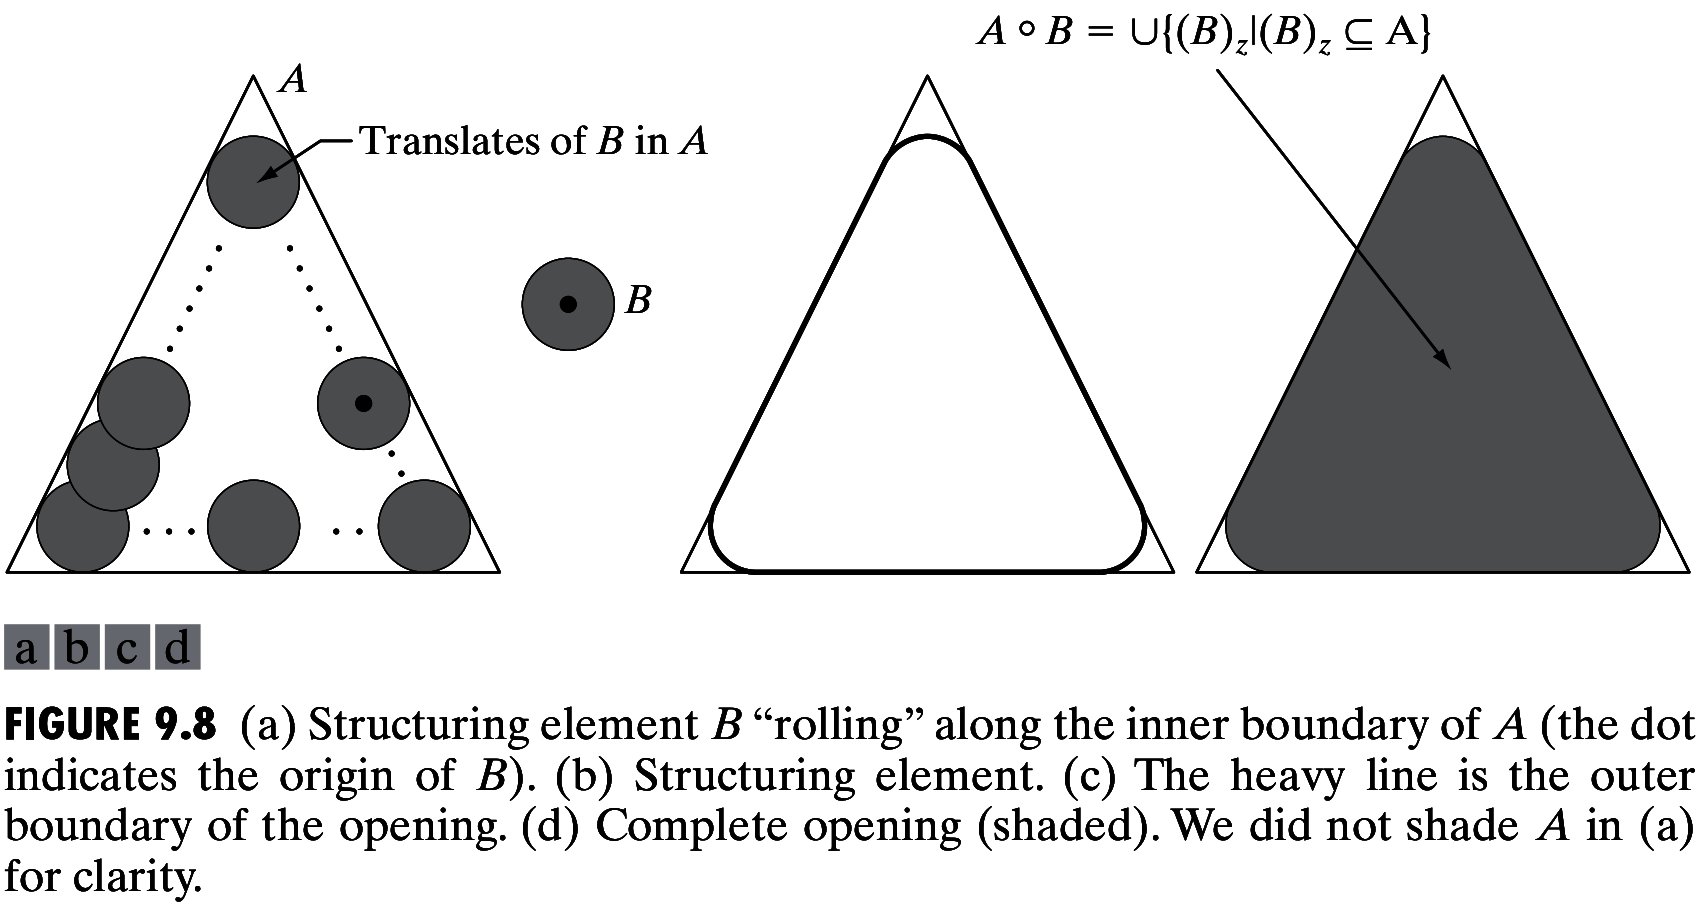
\includegraphics[width=.7\textwidth]{fig-9-8.png}
\end{figure}
\end{frame}

\begin{frame}
\begin{figure}[!h]
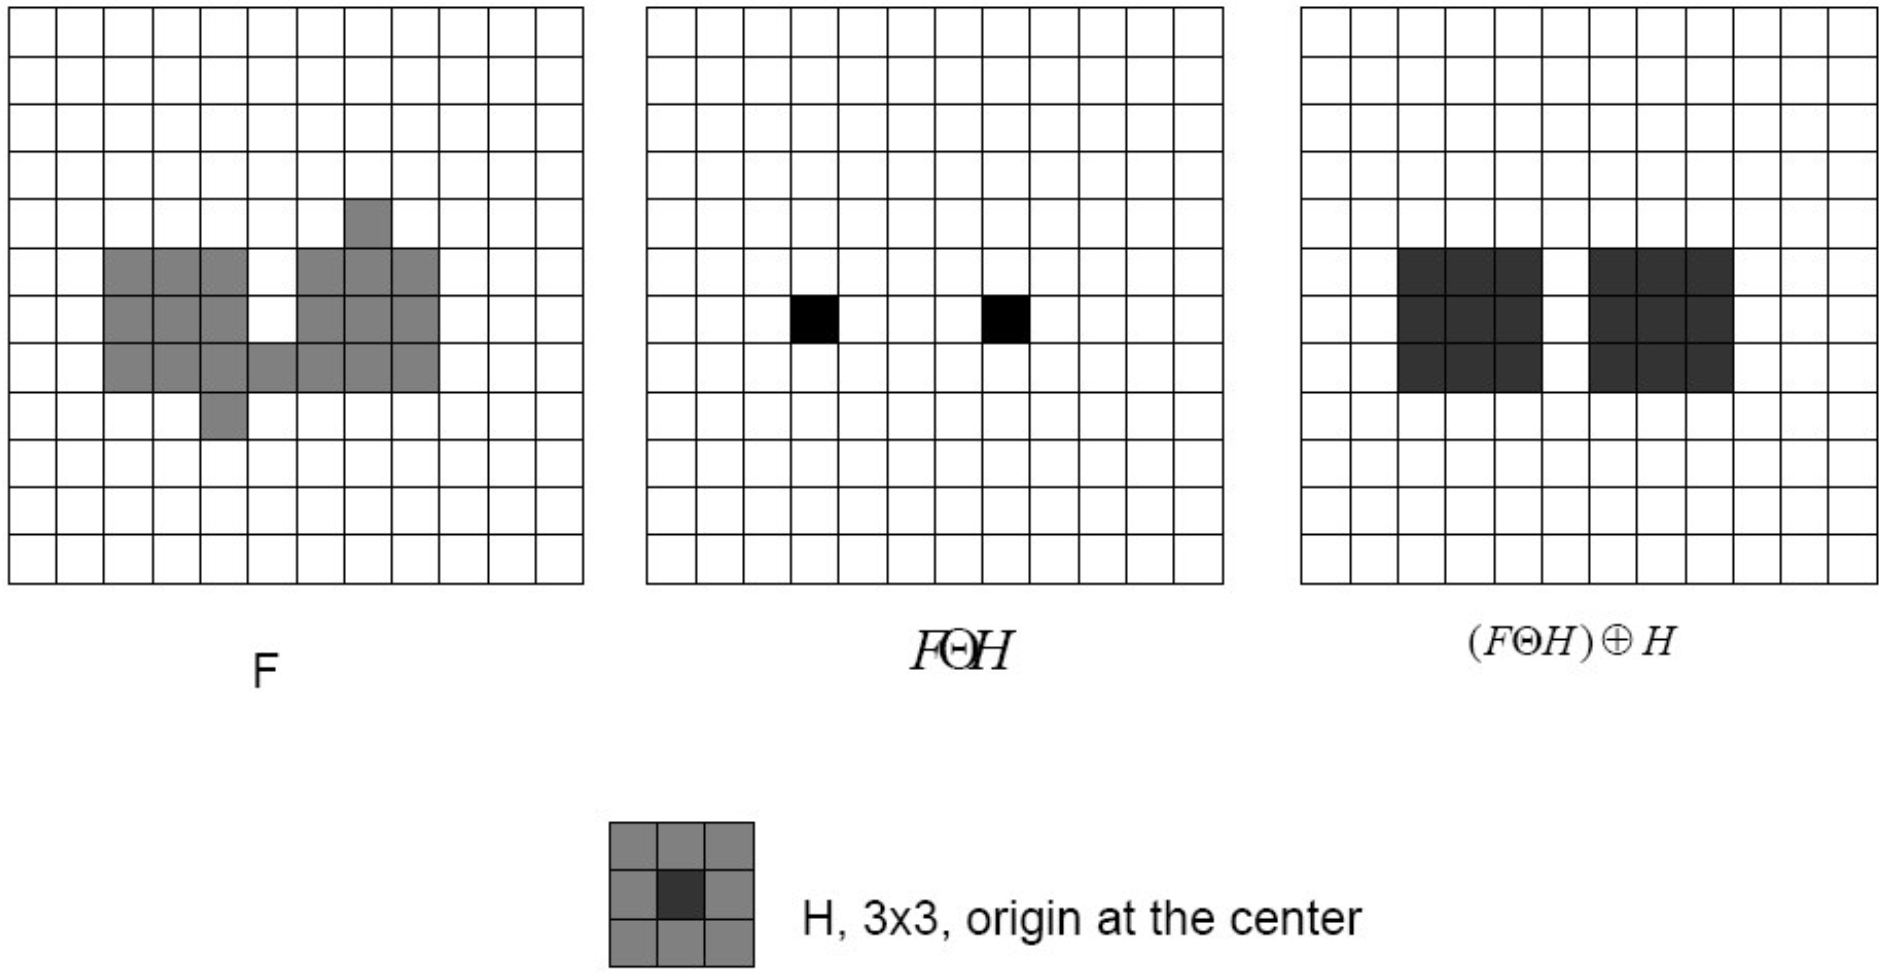
\includegraphics[width=\textwidth]{opening-ex-1.png}
\end{figure}
\end{frame}

\subsection{Closing}

\begin{frame}
\frametitle{Closing}
\begin{columns}
\begin{column}{.3\textwidth}
\begin{figure}
\centering

\includegraphics[width=\textwidth]{closeb.png}
\end{figure}
\end{column}
\begin{column}{.7\textwidth}
\begin{itemize}
\item Dilation followed by an erosion:
\[A \bullet B = \left ( A \oplus B \right ) \ominus B\]
\item Similar to dilation (tends to enlarge foreground boundaries).
\item Less destructive than dilation.
\item Determined by a structuring element (SE).
\end{itemize}
\end{column}
\end{columns}
\end{frame}

\begin{frame}
\begin{columns}
\begin{column}{.3\textwidth}
\begin{figure}
\centering

\includegraphics[width=\textwidth]{closeb.png}
\end{figure}
\end{column}
\begin{column}{.7\textwidth}
Tends to:
\begin{itemize}
\item Preserve background regions that:
\begin{itemize}
\item have similar shape to SE;
\item completely contain the SE.
\end{itemize}
\item Removes regions of the background that cannot contain the SE.
\item Smooths objects contours.
\item Joins narrow breaks.
\item Fills long thing gulfs.
\item Fills holes smaller than the SE.
\end{itemize}
\end{column}
\end{columns}
\end{frame}

\begin{frame}
In closing, the ball $B$ is rolled outside the boundary of $A$:
\begin{figure}[!h]
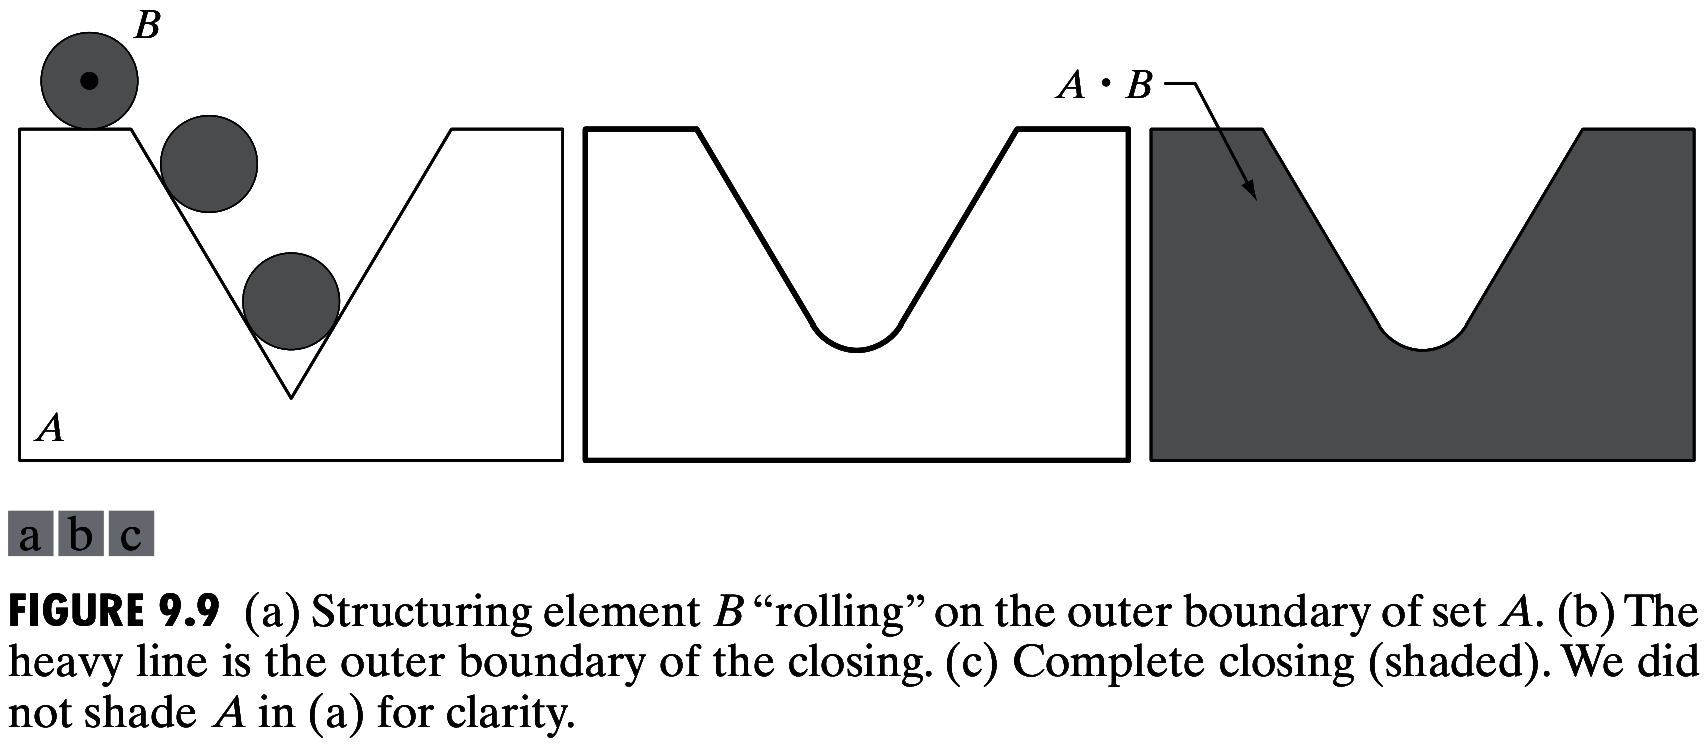
\includegraphics[width=\textwidth]{fig-9-9.png}
\end{figure}
\end{frame}

\begin{frame}
\begin{figure}[!h]
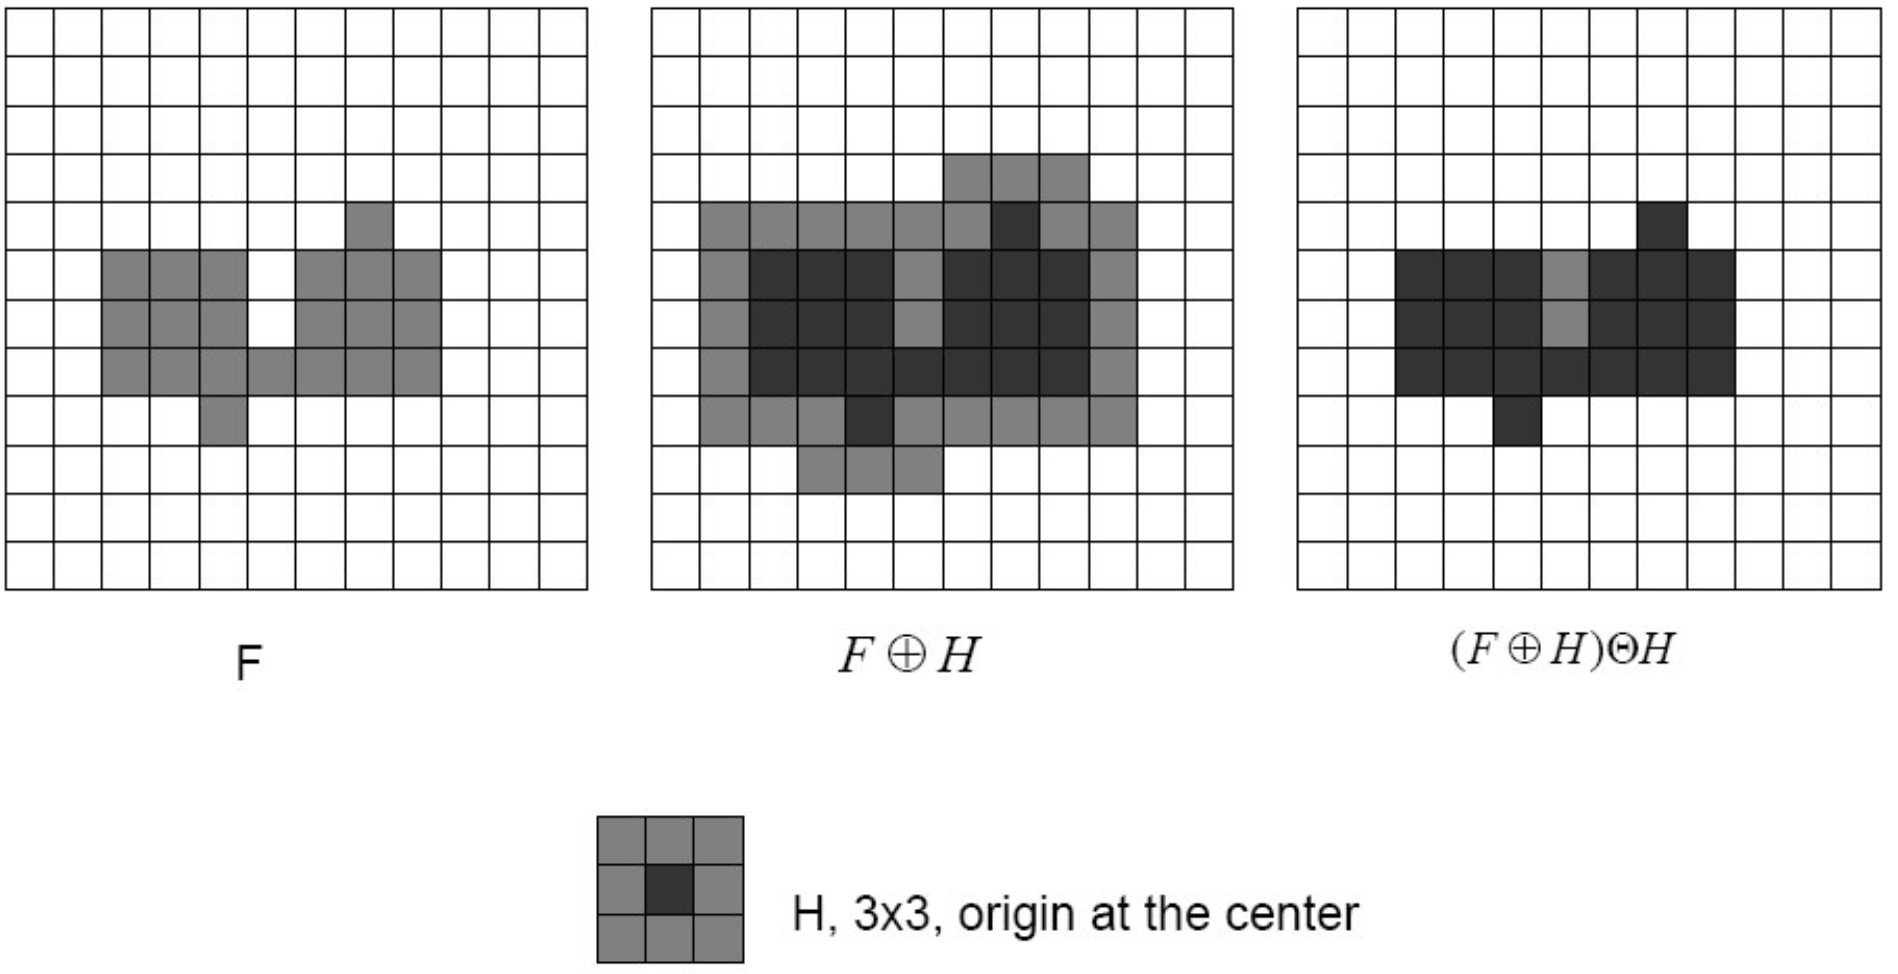
\includegraphics[width=\textwidth]{closing-ex-2.png}
\end{figure}
\end{frame}

\subsection{Opening and closing}

\begin{frame}
\frametitle{Opening and closing}
\begin{figure}[!h]
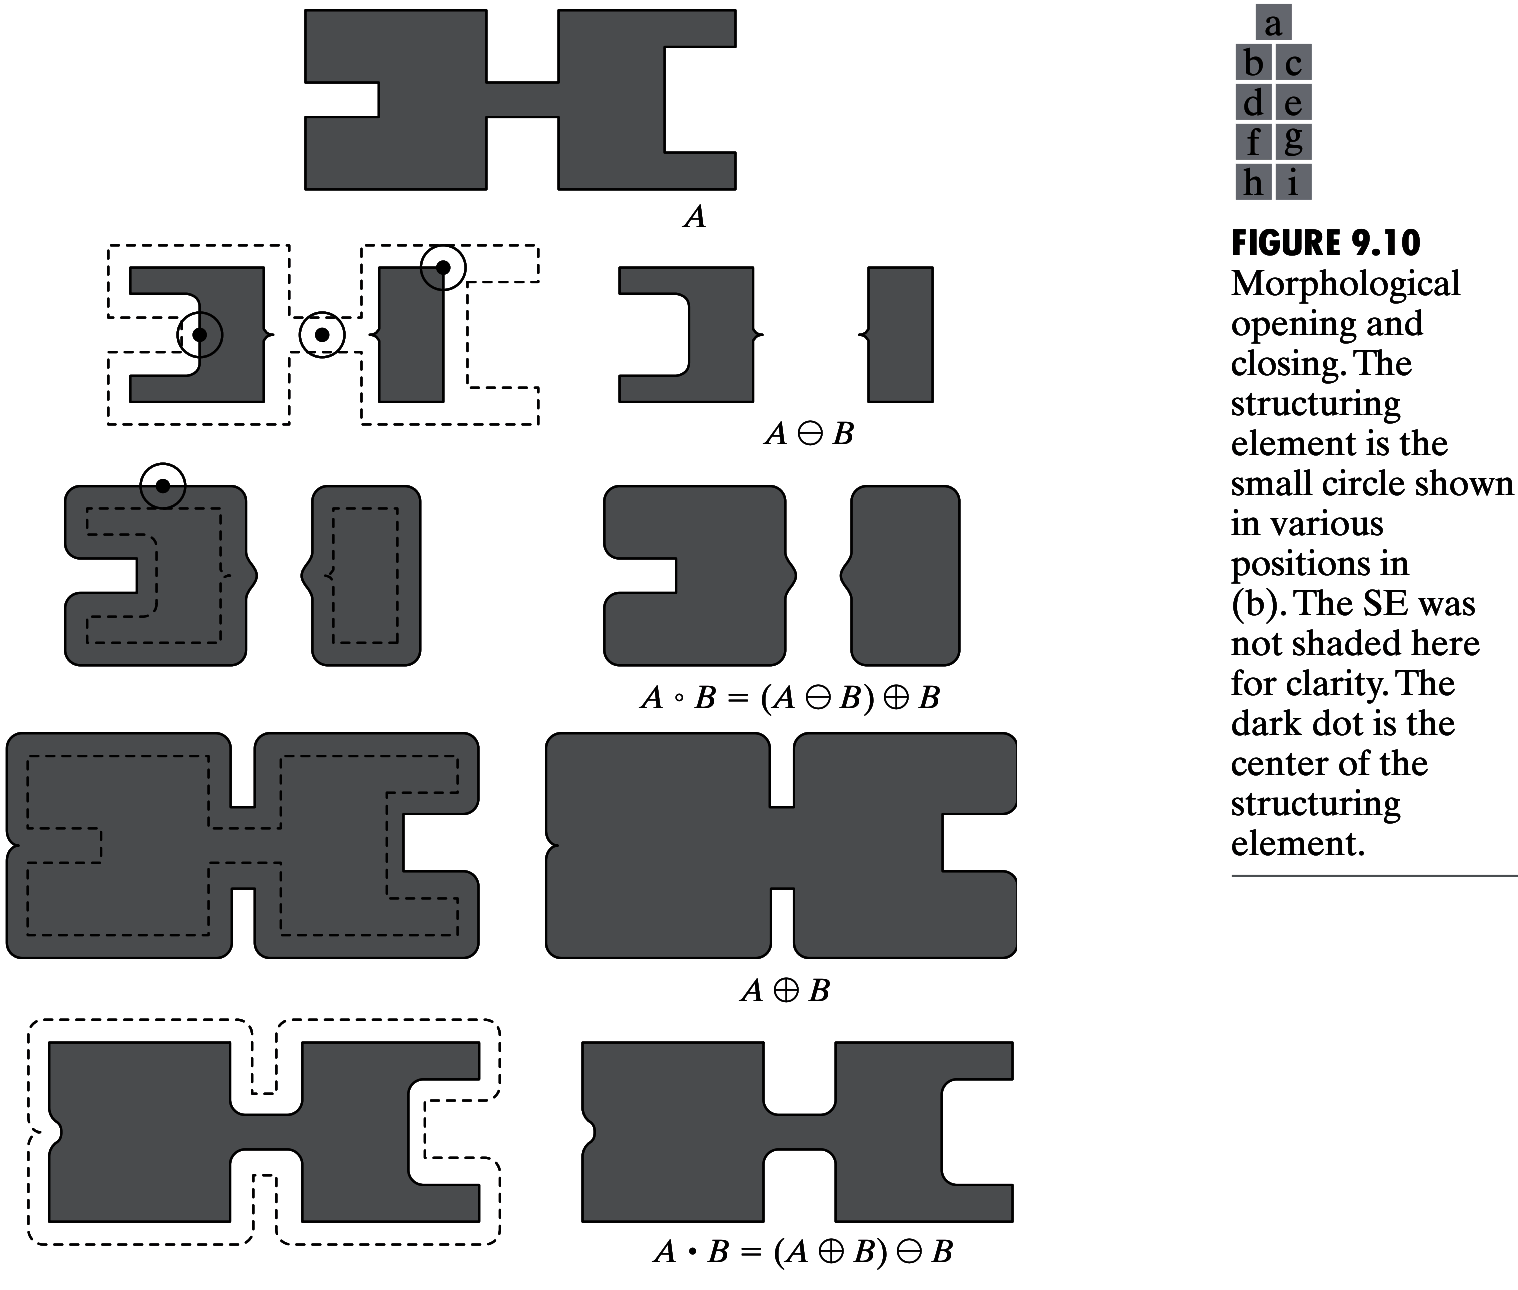
\includegraphics[width=.7\textwidth]{fig-9-10.png}
\end{figure}
\end{frame}

\begin{frame}
\begin{block}{Duality}
Opening and closing are duals of each other wrt. set complementation and reflection:
\begin{itemize}
\item $\left (A \circ B\right )^{c} = A^{c} \bullet \hat{B}$.
\item $\left ( A \bullet B \right )^{c} = A^{c} \circ \hat{B}$.
\end{itemize}
\end{block}
\end{frame}

\begin{frame}
\begin{block}{Properties of opening}
\begin{itemize}
\item $A \circ B$ is a subset of $A$.
\item If $C$ is a subset of $D$, then $C \circ B$ is a subset of $D \circ B$.
\item $\left ( A \circ B \right ) \circ B = A \circ B $.
\end{itemize}
\end{block}
\begin{block}{Properties of closing}
\begin{itemize}
\item $A$ is a subset of $A \bullet B$.
\item If $C$ is a subset of $D$, then $C\bullet B$ is a subset of $D \bullet B$.
\item $ \left ( A\bullet B\right ) \bullet	B = A\bullet B $.
\end{itemize}
\end{block}
\end{frame}

\begin{frame}
Example: Morphological filtering.
\begin{figure}[!h]
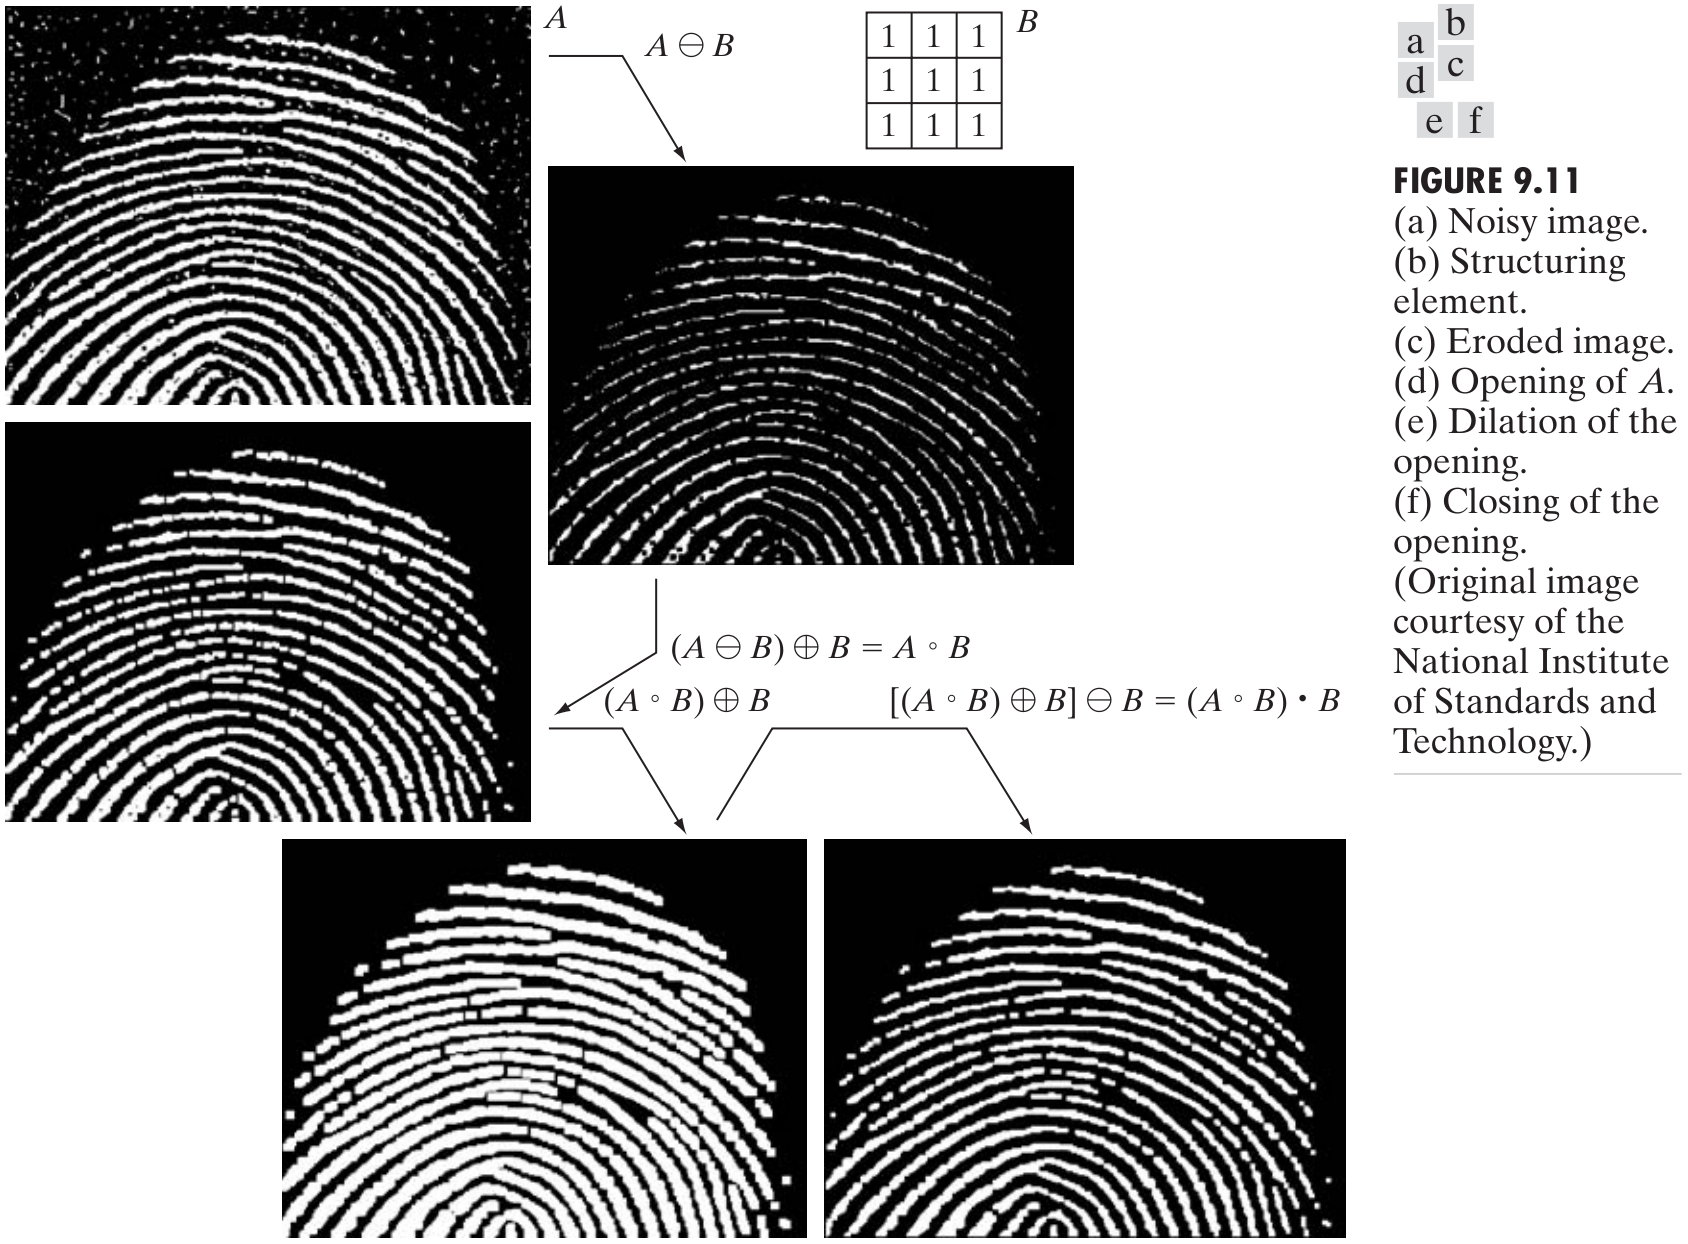
\includegraphics[width=.7\textwidth]{fig-9-11.png}
\end{figure}
\end{frame}

\section{Hit-or-miss transform}

\begin{frame}
\frametitle{Hit-or-miss transform}
\begin{columns}
\begin{column}{.5\textwidth}
The hit-or-miss transform is a basic tool for shape detection.
\begin{block}{Definition}
\[
A \circledast B = \left ( A \ominus B_{1}  \right ) \cap \left ( A^{c} \ominus B_{2} \right )
\]
\[
A \circledast B = \left ( A \ominus B_{1} \right ) - \left ( A \oplus \hat{B}_{2} \right )
\]
\end{block}
\end{column}
\begin{column}{.5\textwidth}
\begin{figure}[!h]
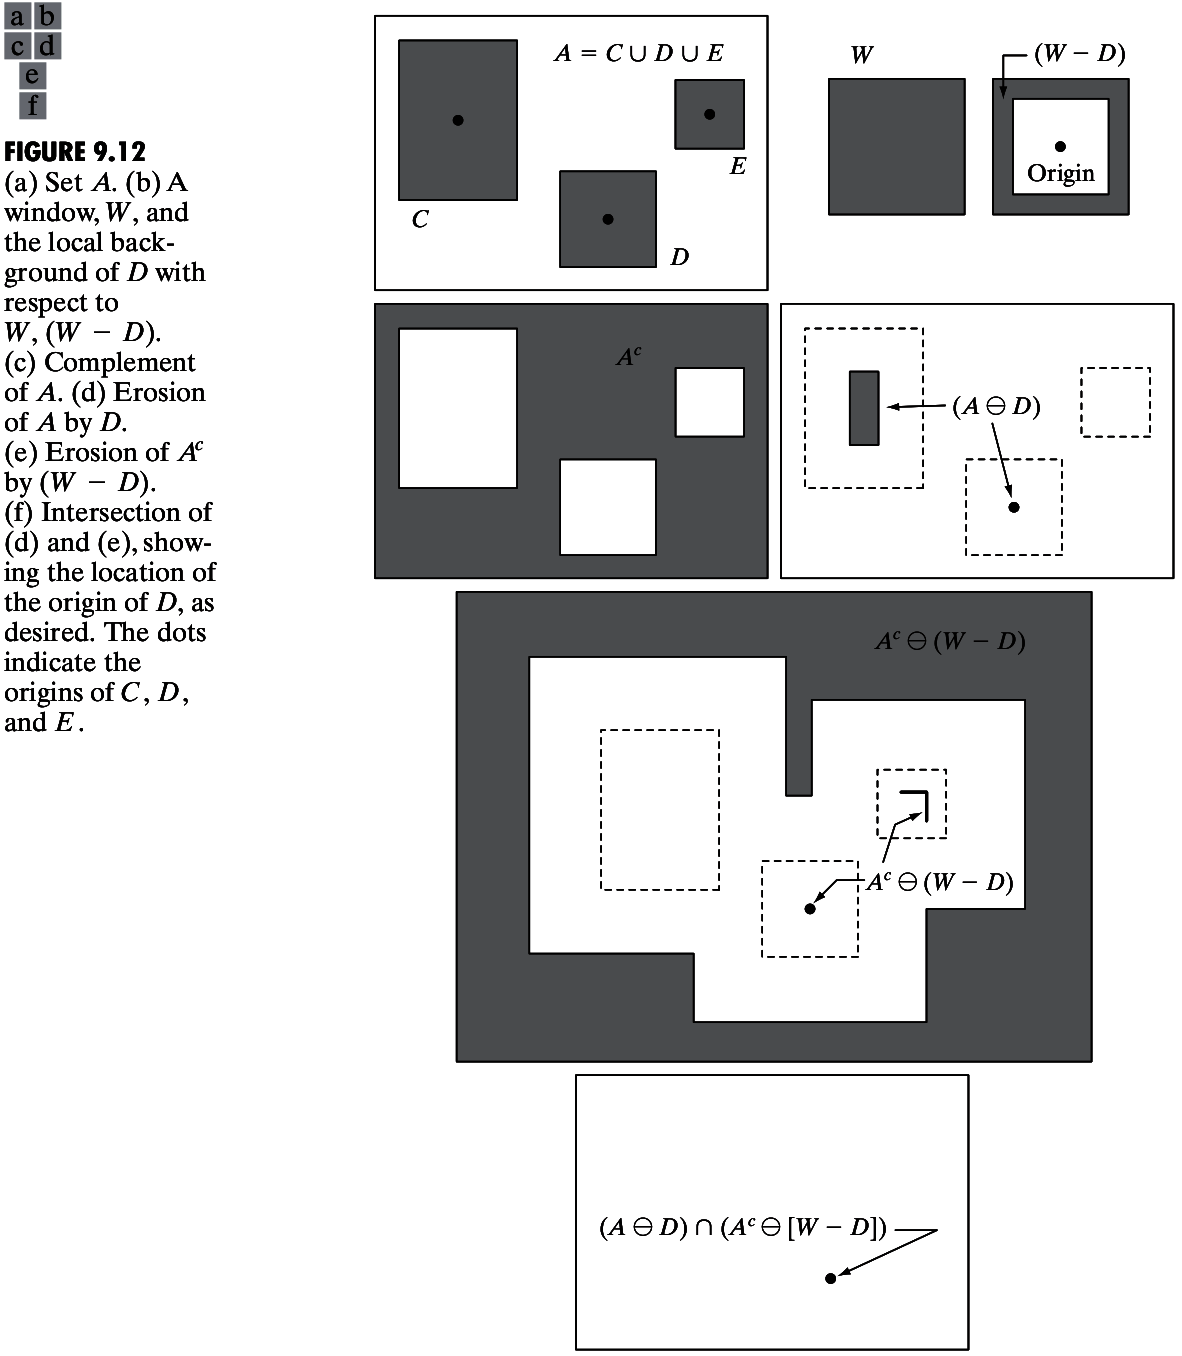
\includegraphics[width=\textwidth]{fig-9-12}
\end{figure}
\end{column}
\end{columns}
\end{frame}

\begin{frame}
Application: Corner detection.
\begin{figure}[!h]
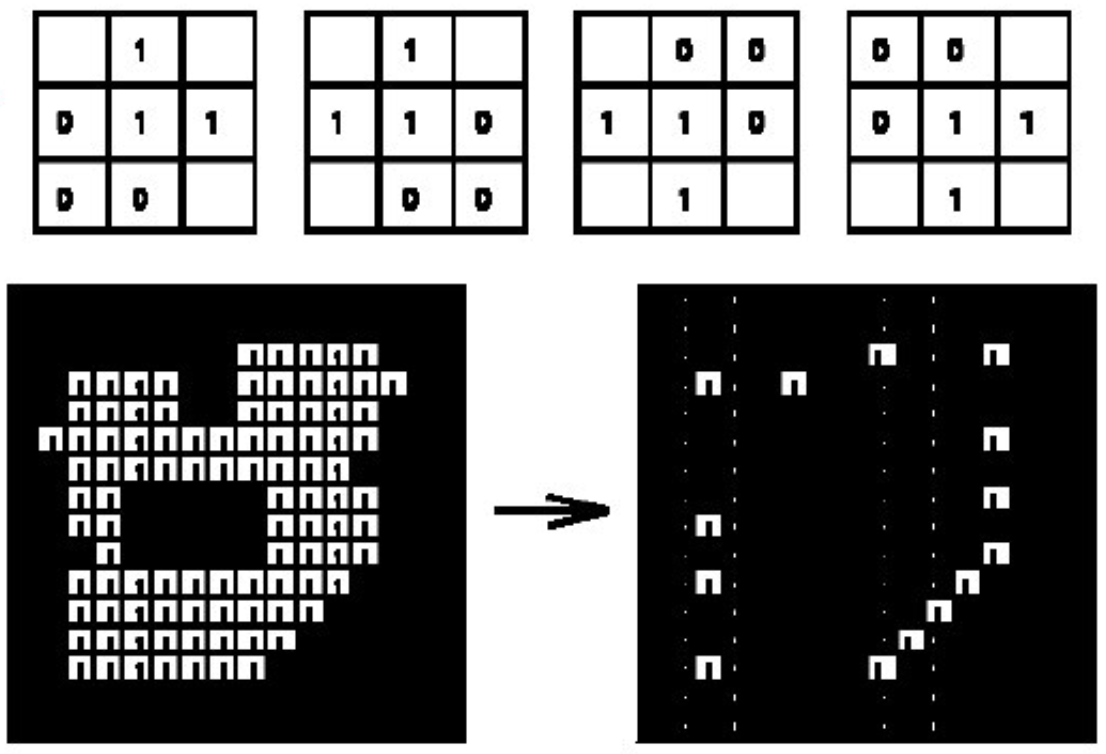
\includegraphics[width=.8\textwidth]{hit-or-miss}
\end{figure}
\end{frame}

\section{Morphological algorithms}

\subsection{Boundary extraction}

\begin{frame}
\frametitle{Boundary extraction}
Definition:
\[
\beta (A) = A - \left  ( A \ominus B \right  )
\]
Using $B = $\texttt{ones(3)}.
\begin{columns}
\begin{column}{.33\textwidth}
\begin{figure}
\centering
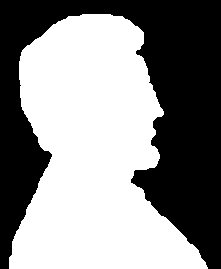
\includegraphics[width=.6\textwidth]{A.png}
\caption{A}
\end{figure}
\end{column}
\begin{column}{.33\textwidth}
\begin{figure}
\centering
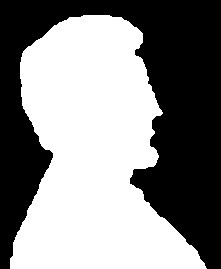
\includegraphics[width=.6\textwidth]{B.png}
\caption{$A\ominus B$}
\end{figure}
\end{column}
\begin{column}{.33\textwidth}
\begin{figure}
\centering
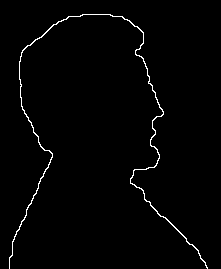
\includegraphics[width=.6\textwidth]{beta.png}
\caption{$\beta$}
\end{figure}
\end{column}
\end{columns}
\end{frame}

\subsection{Hole filling}

\begin{frame}
\frametitle{Hole filling}
Iterations:
$X_{k} = \left ( X_{k-1} \oplus B \right ) \cap A^{c}\ \ \ k=1,2,\ldots$
\begin{columns}
\begin{column}{.45\textwidth}
\begin{figure}[!h]
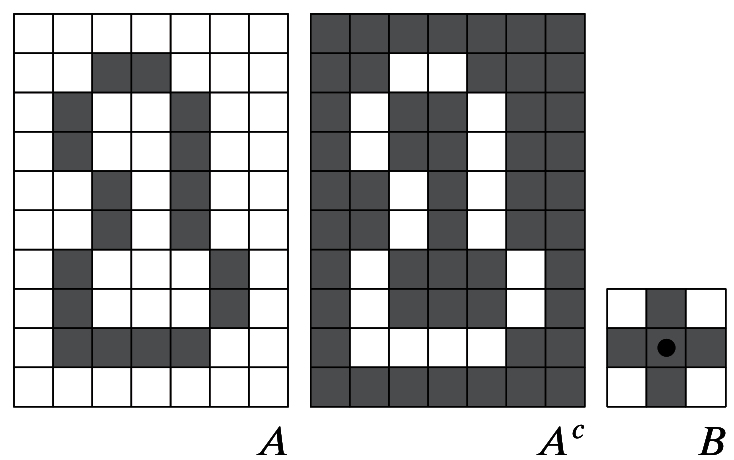
\includegraphics[width=\textwidth]{fig-9-15abc.png}
\end{figure}
\end{column}
\begin{column}{.55\textwidth}
\begin{figure}[!h]
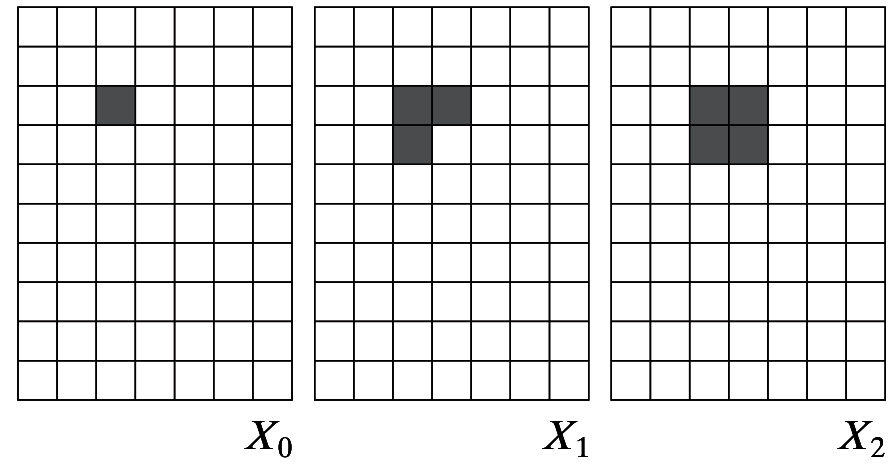
\includegraphics[width=\textwidth]{fig-9-15def.png}
\end{figure}
\end{column}
\end{columns}
\end{frame}

\begin{frame}
Result:
\begin{columns}
\begin{column}{.45\textwidth}
\begin{figure}[!h]
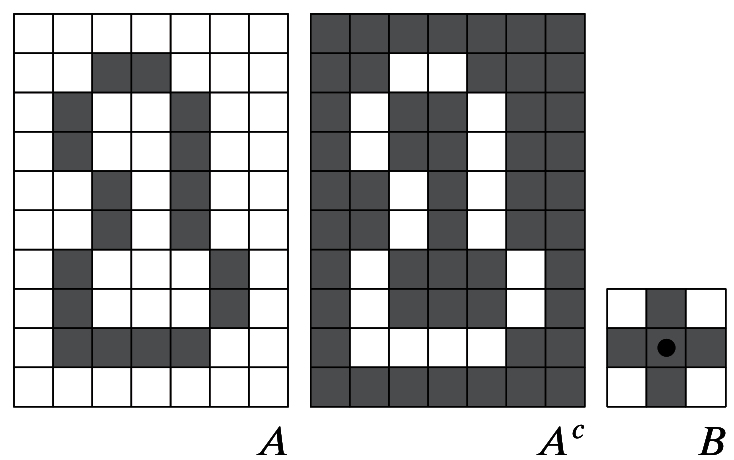
\includegraphics[width=\textwidth]{fig-9-15abc.png}
\end{figure}
\end{column}
\begin{column}{.55\textwidth}
\begin{figure}[!h]
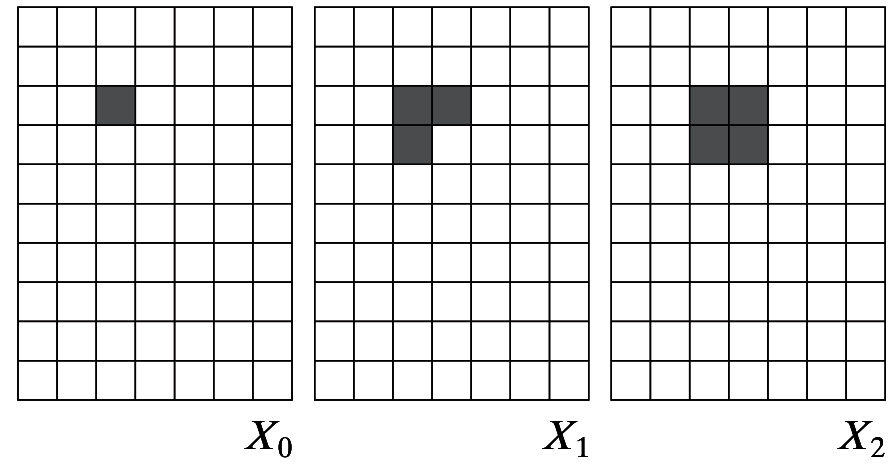
\includegraphics[width=\textwidth]{fig-9-15def.png}
\end{figure}
\end{column}
\end{columns}
\begin{figure}[!h]
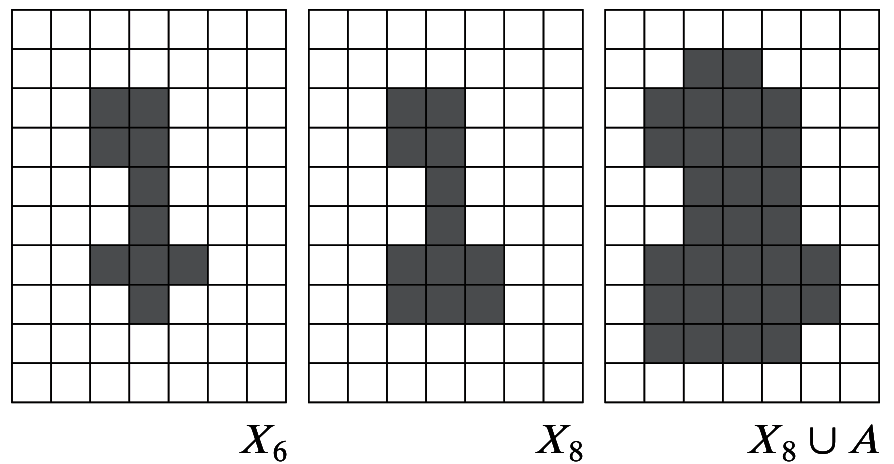
\includegraphics[width=.5\textwidth]{fig-9-15ghi.png}
\end{figure}
\end{frame}

\begin{frame}
Example: Morphological hole filling:
\begin{figure}[!h]
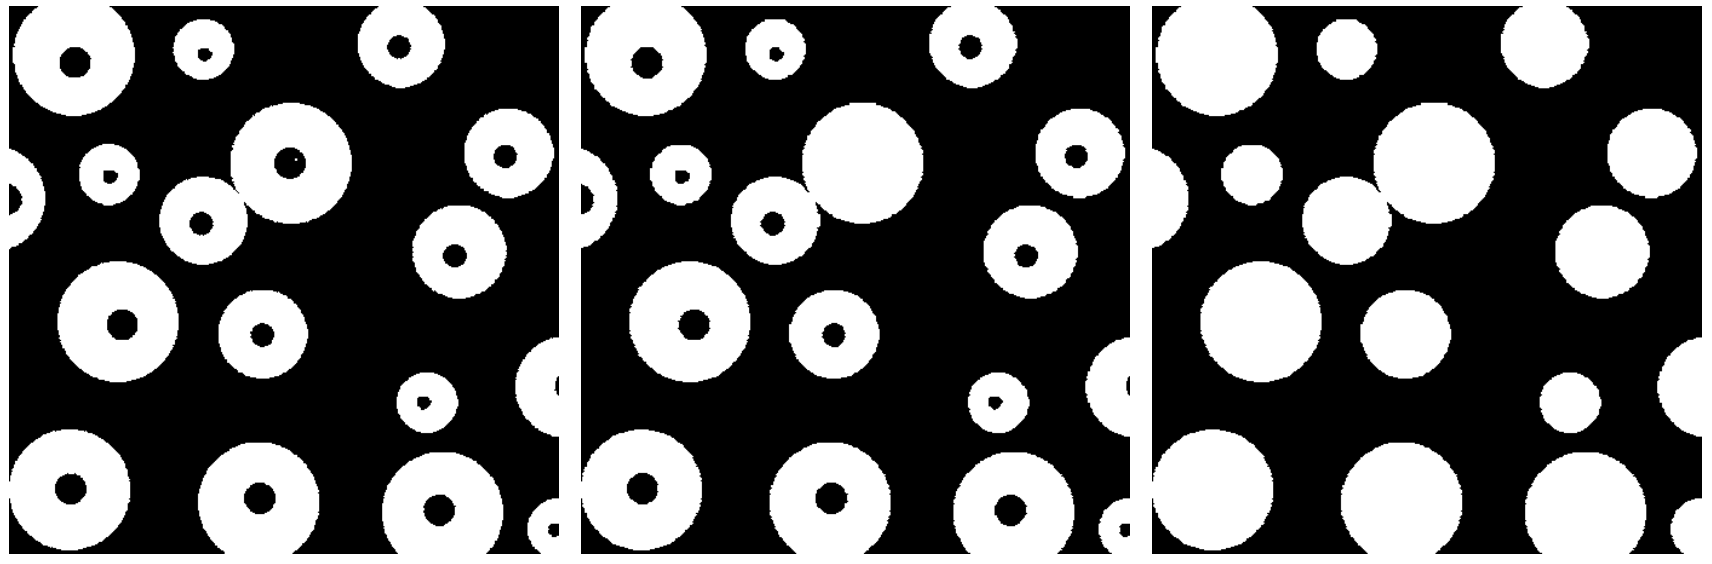
\includegraphics[width=\textwidth]{ex-9-16.png}
\end{figure}
\end{frame}

\subsection{Extraction of connected components}

\begin{frame}
\frametitle{Extraction of connected components}
Iterations $X_{k} = \left ( X_{k-1} \oplus B \right ) \cap A\ \ \ k=1,2,\ldots$
\begin{figure}[!h]
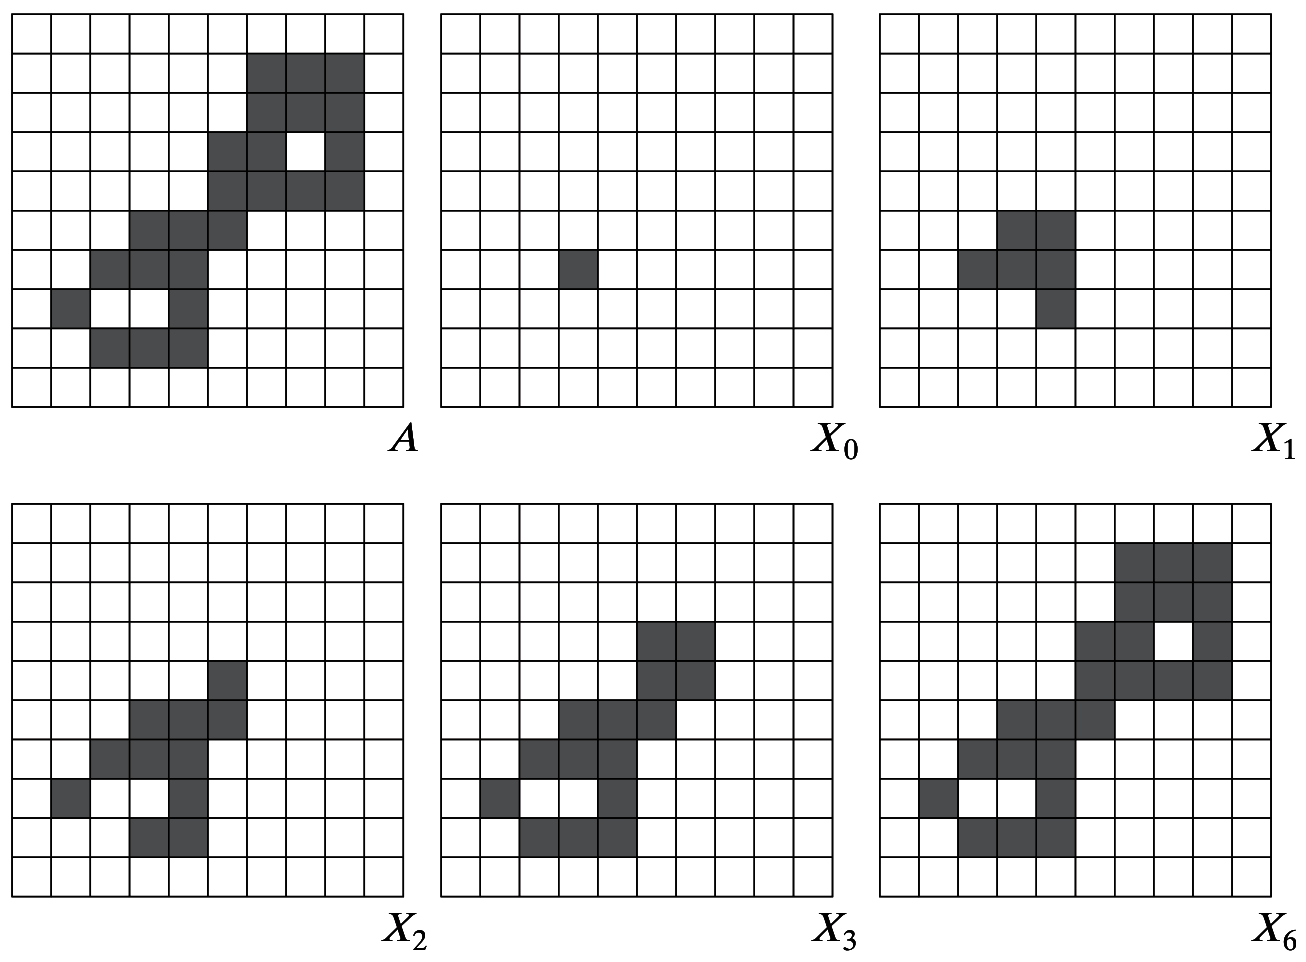
\includegraphics[width=.7\textwidth]{fig-9-17}
\end{figure}
\end{frame}

\begin{frame}
Ex 9.7: Detecting foreign objects in packaged food.
\begin{columns}
\begin{column}{.6\textwidth}
\begin{figure}[!h]
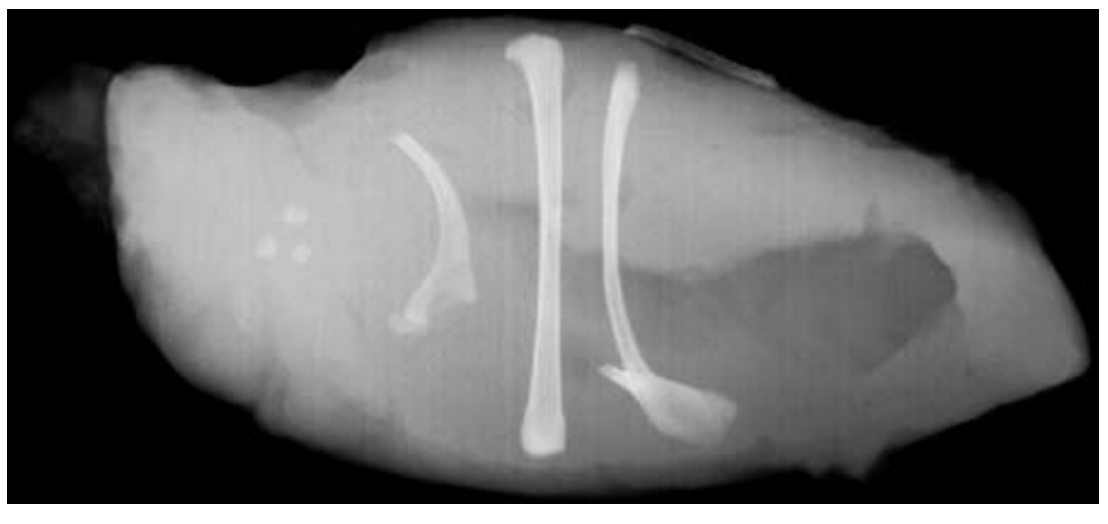
\includegraphics[width=.6\textwidth]{fig-9-18a.png}
\caption{Chicken breast with bone fragments.}
\end{figure}
\begin{figure}[!h]
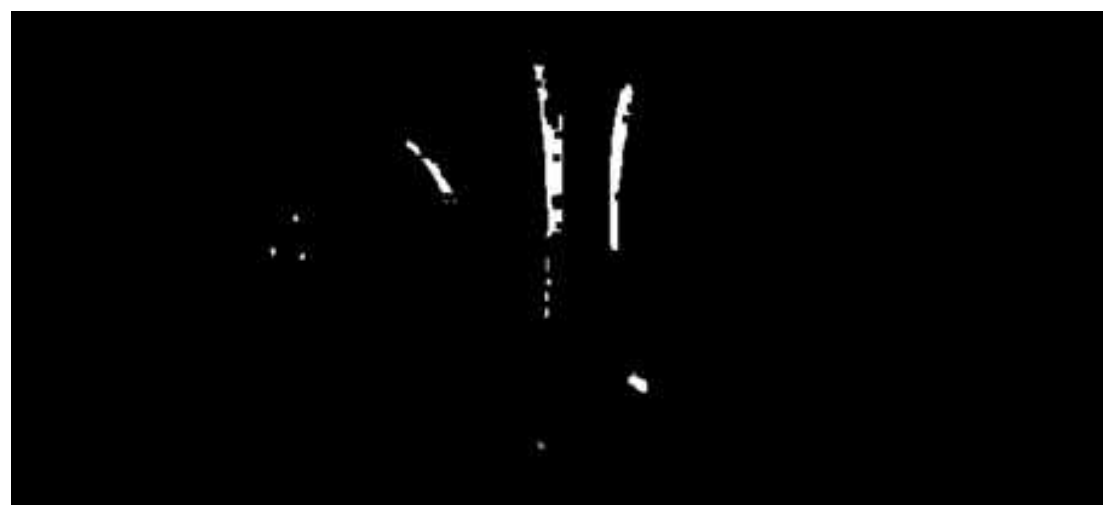
\includegraphics[width=.6\textwidth]{fig-9-18c.png}
\caption{Threshold and erosion of original.}
\end{figure}
\end{column}
\begin{column}{.3\textwidth}
\begin{figure}[!h]
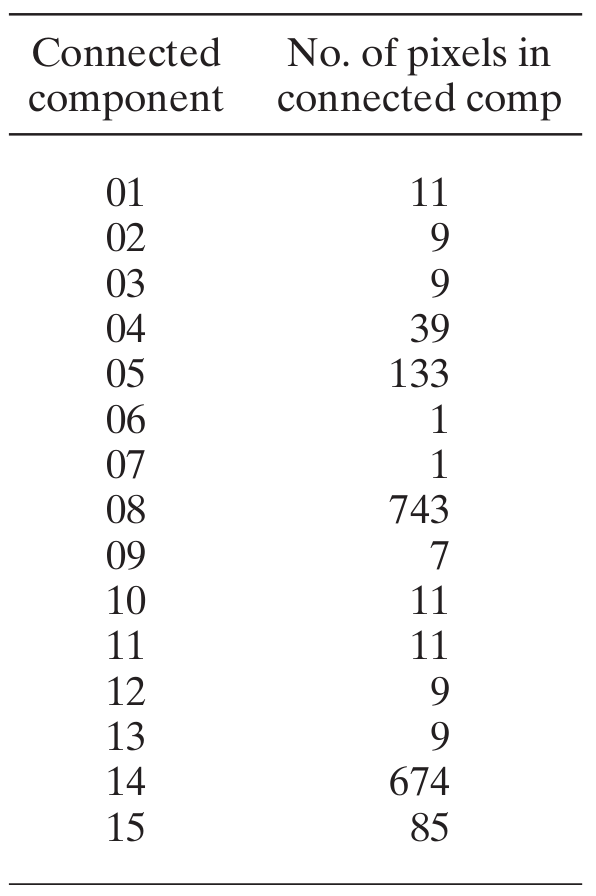
\includegraphics[width=\textwidth]{fig-9-18d.png}
\end{figure}
\end{column}
\end{columns}
\end{frame}

\subsection{Convex hull}

\begin{frame}
\frametitle{Convex hull}
\begin{itemize}
\item A set $A$ is \textit{convex} if a line segment joining any two points in $A$ lies entirely within $A$.
\item The convex \textit{hull} $H$ of set $S$ is the smallest convex set containing $S$.
\item The set difference is called the convex deficiency of $S$.
\item Useful for description.
\end{itemize}
\begin{figure}[!h]
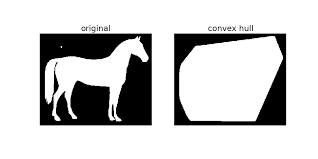
\includegraphics[width=.7\textwidth]{convhull}
\end{figure}
\end{frame}

\begin{frame}
\begin{columns}
\begin{column}{.4\textwidth}
$X_{k}^{i} = \left ( X_{k-1} \circledast B^{i} \right ) \cup A$\\
Four SEs $B^{i}$.\\
$i=1,\ldots 4$.\\
$k = 1, 2,\ldots$\\
$X_{0}^{i} = A$.\\
When $X_{k}^{i} = X_{k-1}^{i}$ we let $D^{i} = X_{k}^{i}$.\\
Final convex hull:\\
$C(A) = \bigcup_{i=1}^{4} D^{i}$.\\
MATLAB = \texttt{convhull}.
\end{column}
\begin{column}{.6\textwidth}
\begin{figure}[!h]
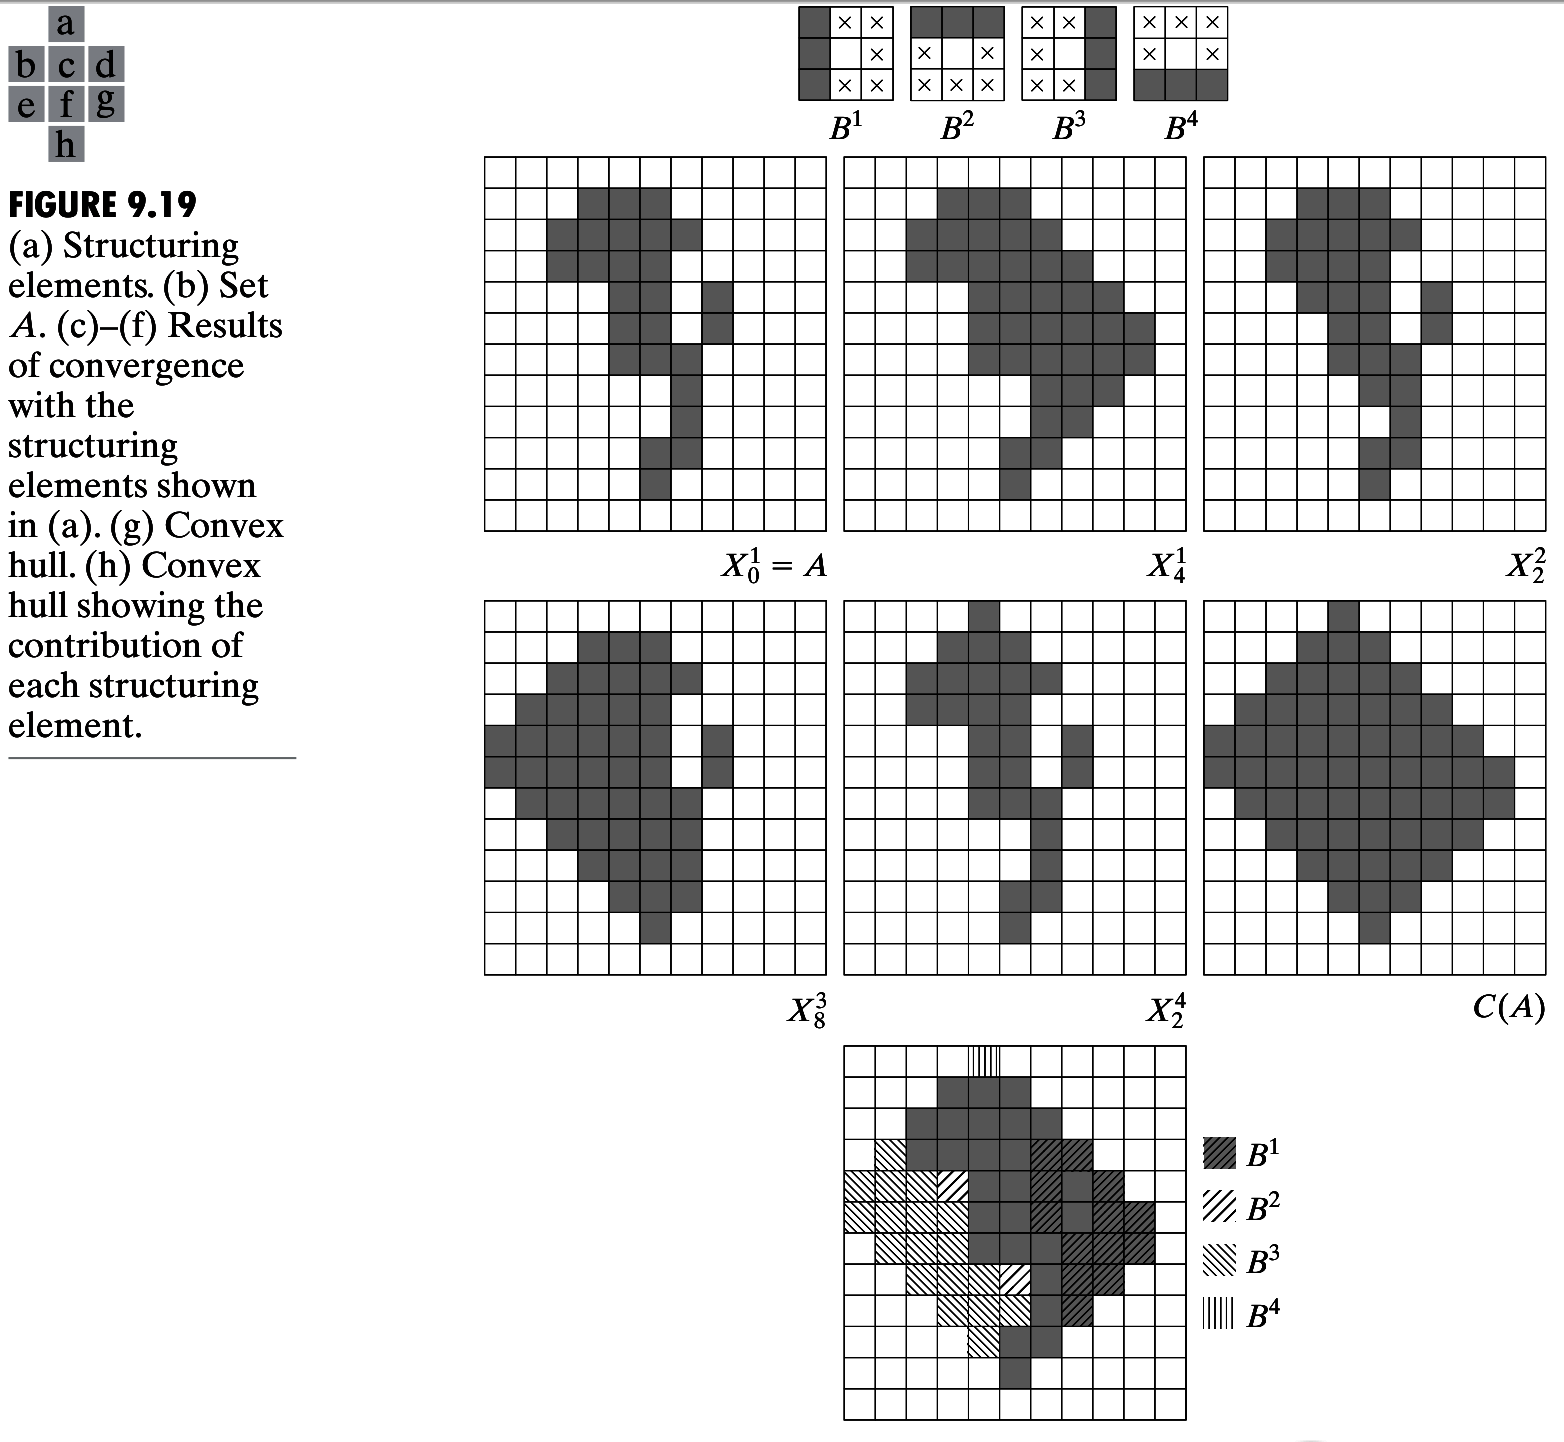
\includegraphics[width=.95\textwidth]{fig-9-19}
\end{figure}
\end{column}
\end{columns}
\end{frame}

\begin{frame}
Limit growth beyond the minimum dimensions guaranteeing convexity.
\begin{figure}[!h]
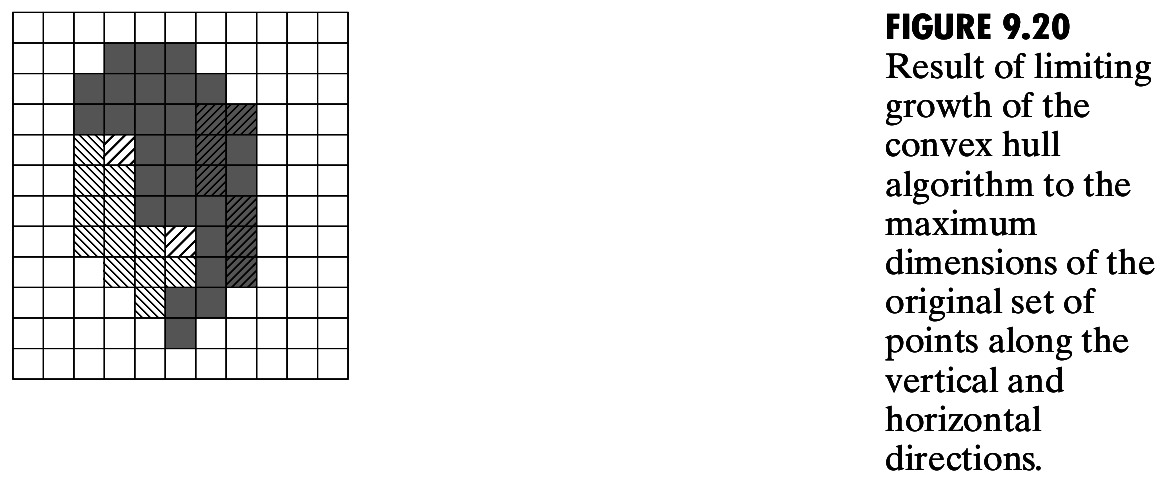
\includegraphics[width=\textwidth]{fig-9-20}
\end{figure}
\end{frame}

\subsection{Thinning}

\begin{frame}
\frametitle{Thinning}
\begin{columns}
\begin{column}{.4\textwidth}
\scriptsize
Thinning of set $A$ by SE $B$ is defined as
\[
A \otimes B = A - \left ( A \circledast B  \right )
\]
\[
A \otimes B = A \cap \left ( A \circledast B \right )^{c}.
\]
\begin{itemize}
\item No background operation is required (we want only hits).
\item Sequence of SEs:
\[
\left \{ B \right \} = \left \{ B^{1}, B^{2}, \ldots, B^{n} \right \}.
\]
\end{itemize}
%\[
%A \otimes B = A \cap \left ( A \circledast B \right )^{c}
%\]
\[
A \otimes \{B\} = ((\ldots ((A\otimes B^{1} ) \otimes B^{2} ) \ldots ) \otimes B^{n})
\]
\normalsize
\end{column}
\begin{column}{.6\textwidth}
\begin{figure}[!h]
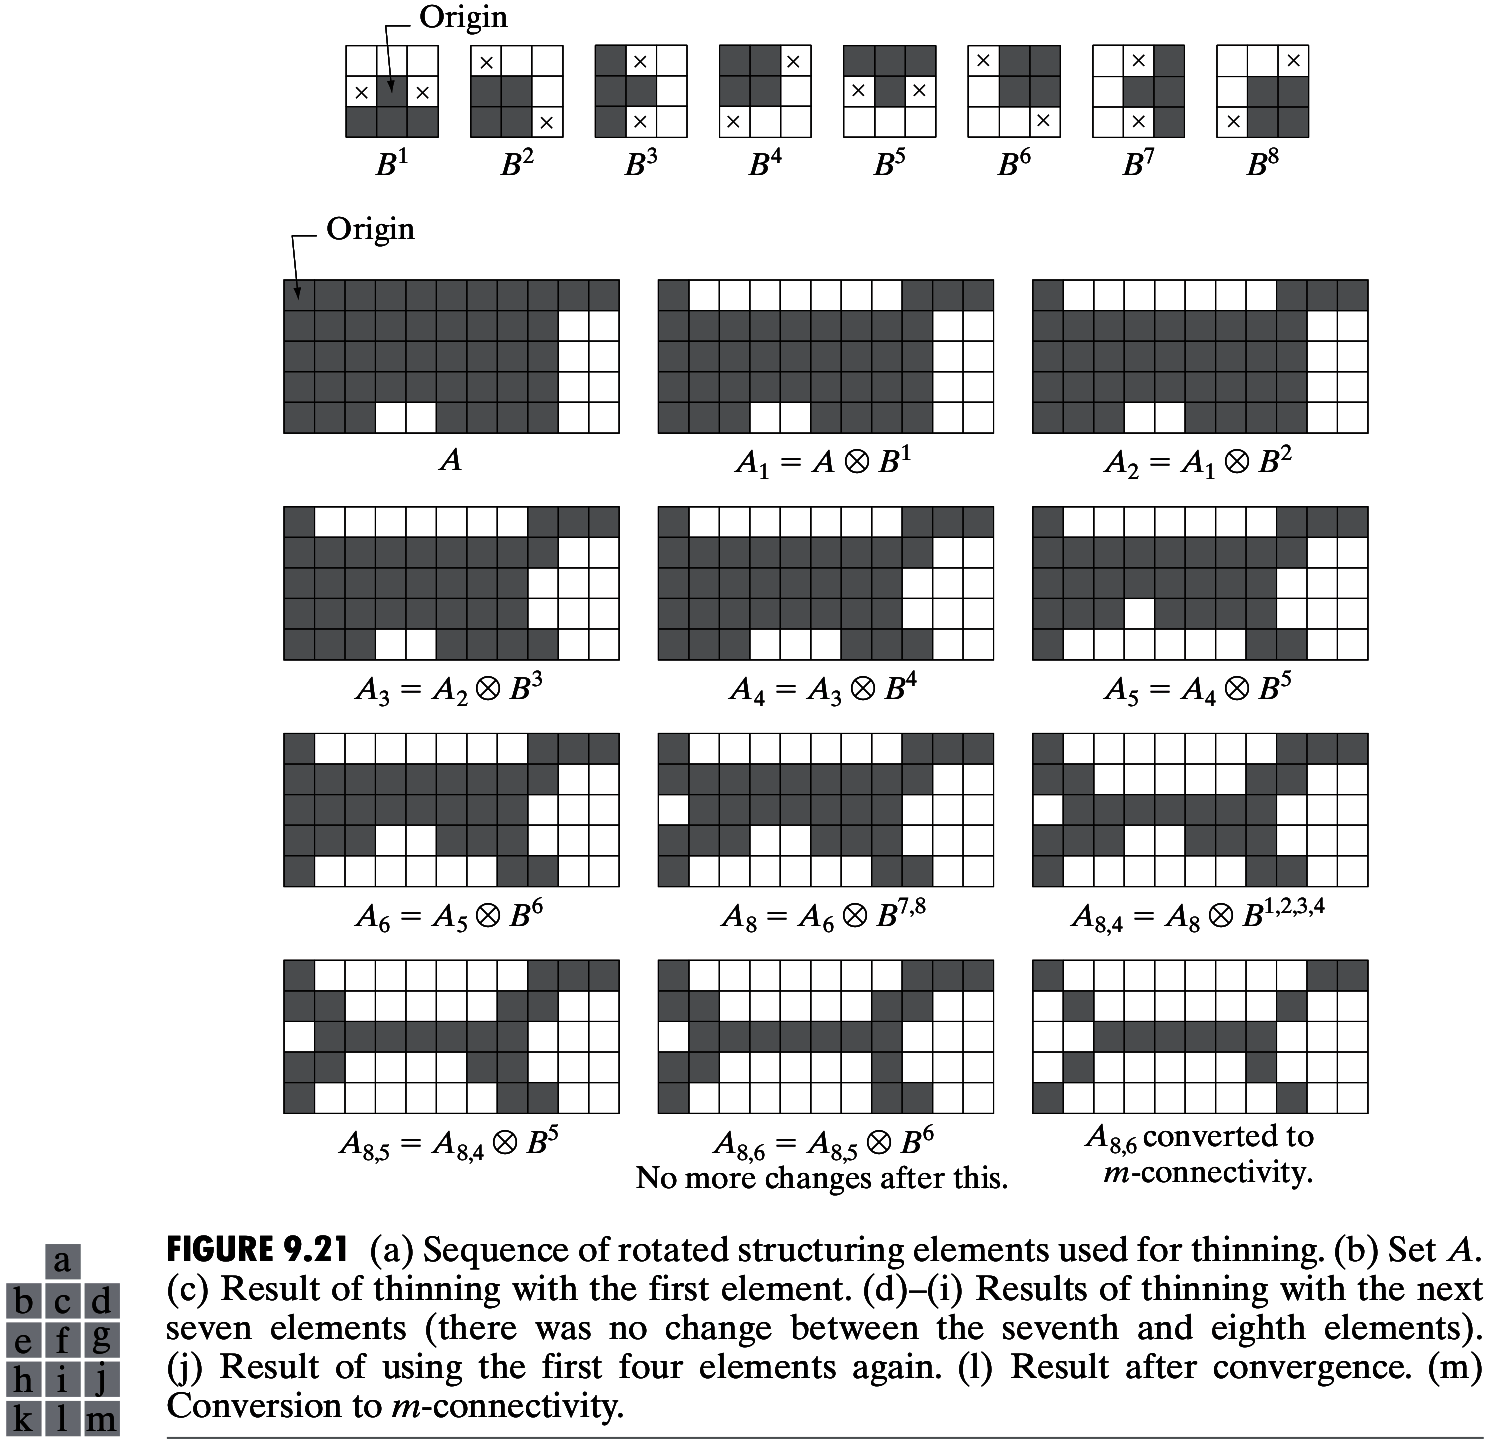
\includegraphics[width=\textwidth]{fig-9-21.png}
\end{figure}
\end{column}
\end{columns}
\end{frame}

\subsection{Thickening}

\begin{frame}
\frametitle{Thickening}
\begin{columns}
\begin{column}{.5\textwidth}
\scriptsize
Thickening is defined as
$A  \odot  B = A \cup (A \circledast B )$
$A  \odot  \{B\} = ((\ldots ((A  \odot  B^{1} )  \odot  B^{2} ) \ldots )  \odot  B^{n})$\\
In practice:\\
$A  \odot  \{B\} = (A^{c} \otimes \{B\})^{c}$.
then post process to remove disconnected points.
\normalsize
\end{column}
\begin{column}{.5\textwidth}
\begin{figure}[!h]
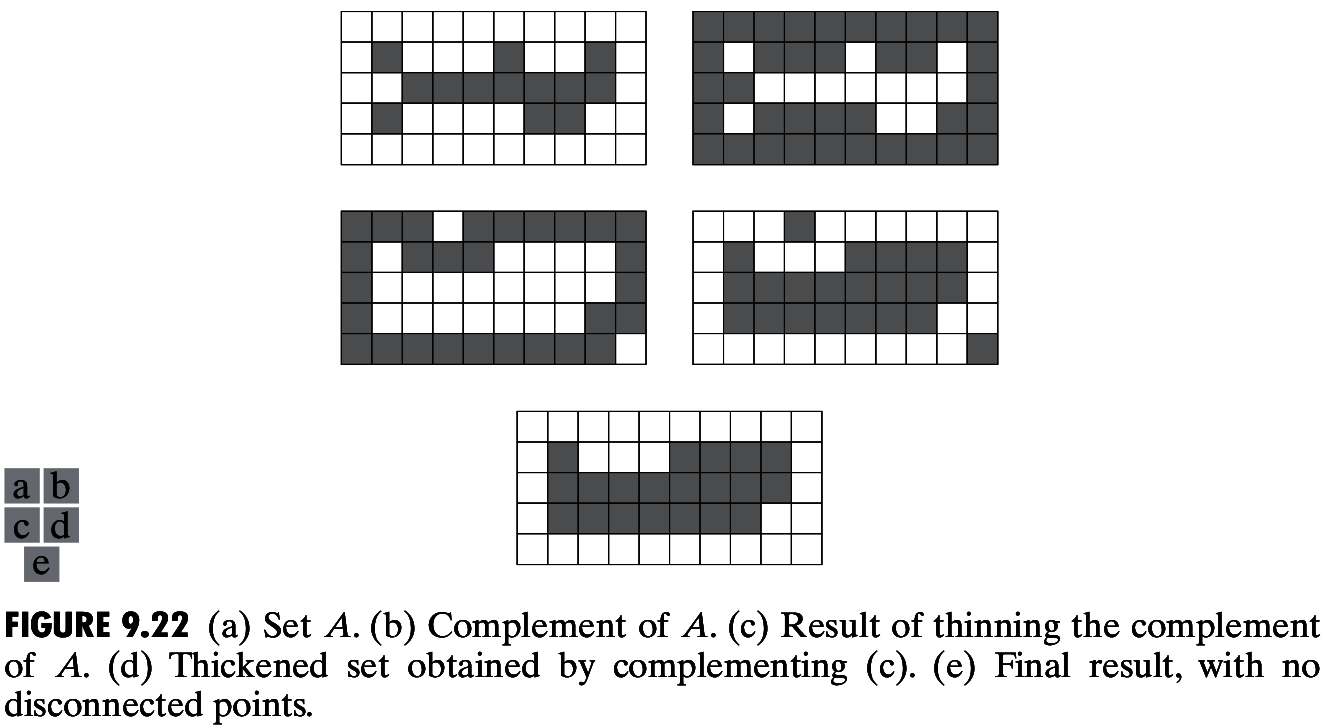
\includegraphics[width=\textwidth]{fig-9-22.png}
\end{figure}
\end{column}
\end{columns}
\end{frame}

\subsection{Skeletons}

\begin{frame}
\frametitle{Skeletons}
\begin{figure}[!h]
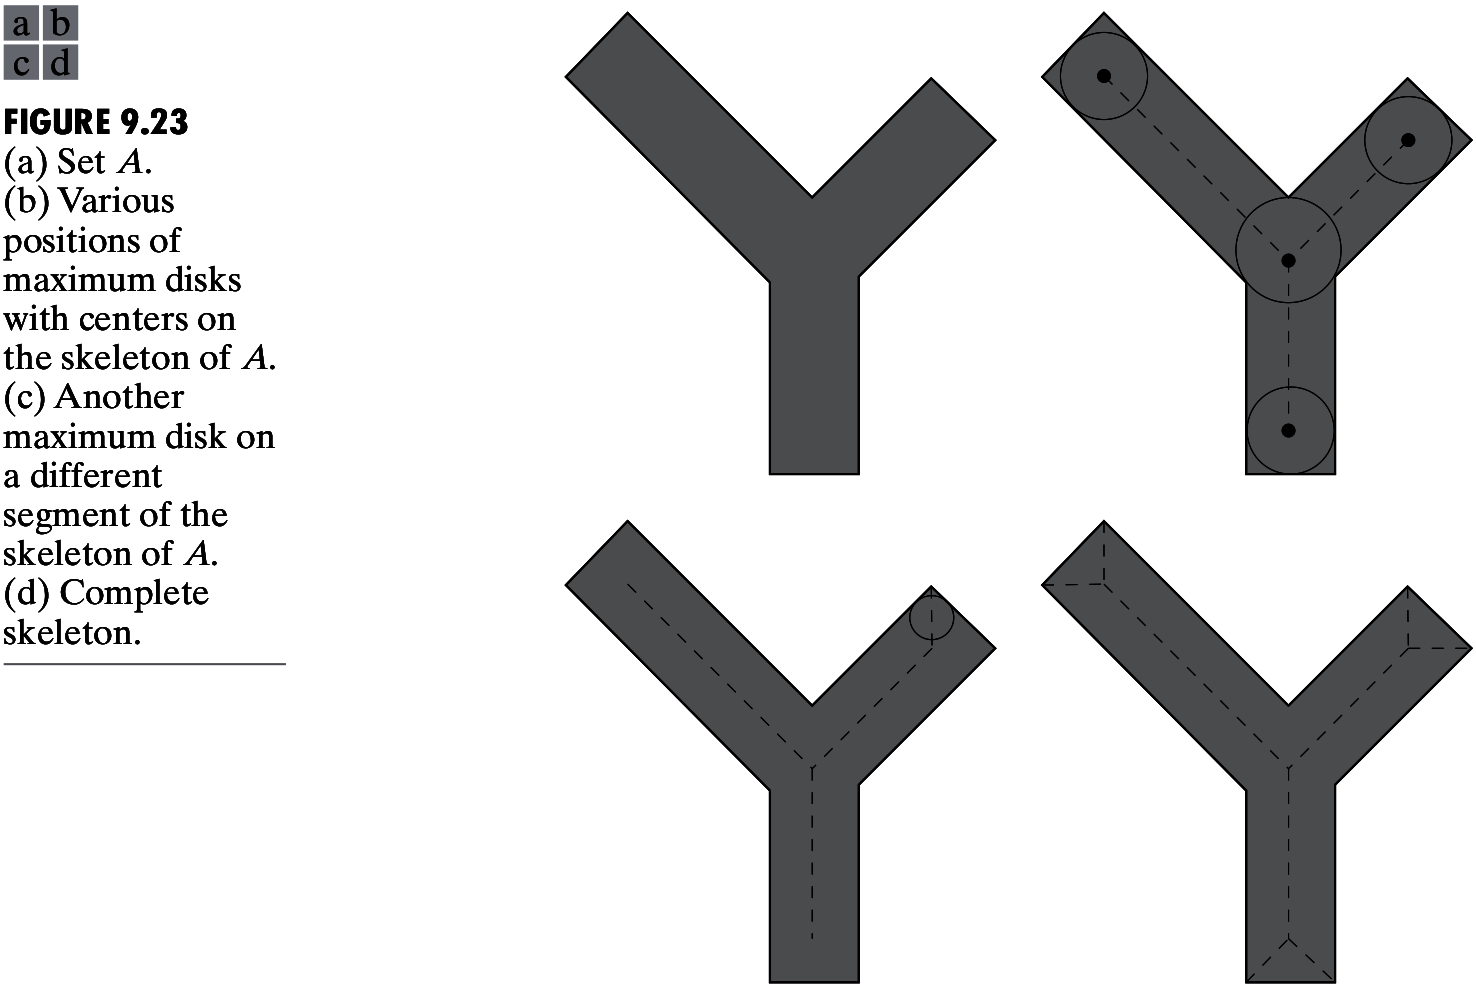
\includegraphics[width=.6\textwidth]{fig-9-23.png}
\end{figure}
\end{frame}

\begin{frame}
The skeleton can be expressed in terms of erosions and openings
$S(A) = \bigcup_{k=0}^{K} S_{k}(A)$\\
where\\
\begin{itemize}
\item $S_{k}(A) = ( A \ominus k B ) - ( A \ominus k B ) \circ B $
\item $A \ominus kB = (( \ldots ((A \ominus B ) \ominus B ) \ominus \ldots ) \ominus B )$ $k$ times.
\end{itemize}
Also, $A$ can be reconstructed using\\
$A = \bigcup_{k-0}^{K} \left ( S_{k}(A) \oplus kB \right )$
\end{frame}

\begin{frame}
\begin{figure}[!h]
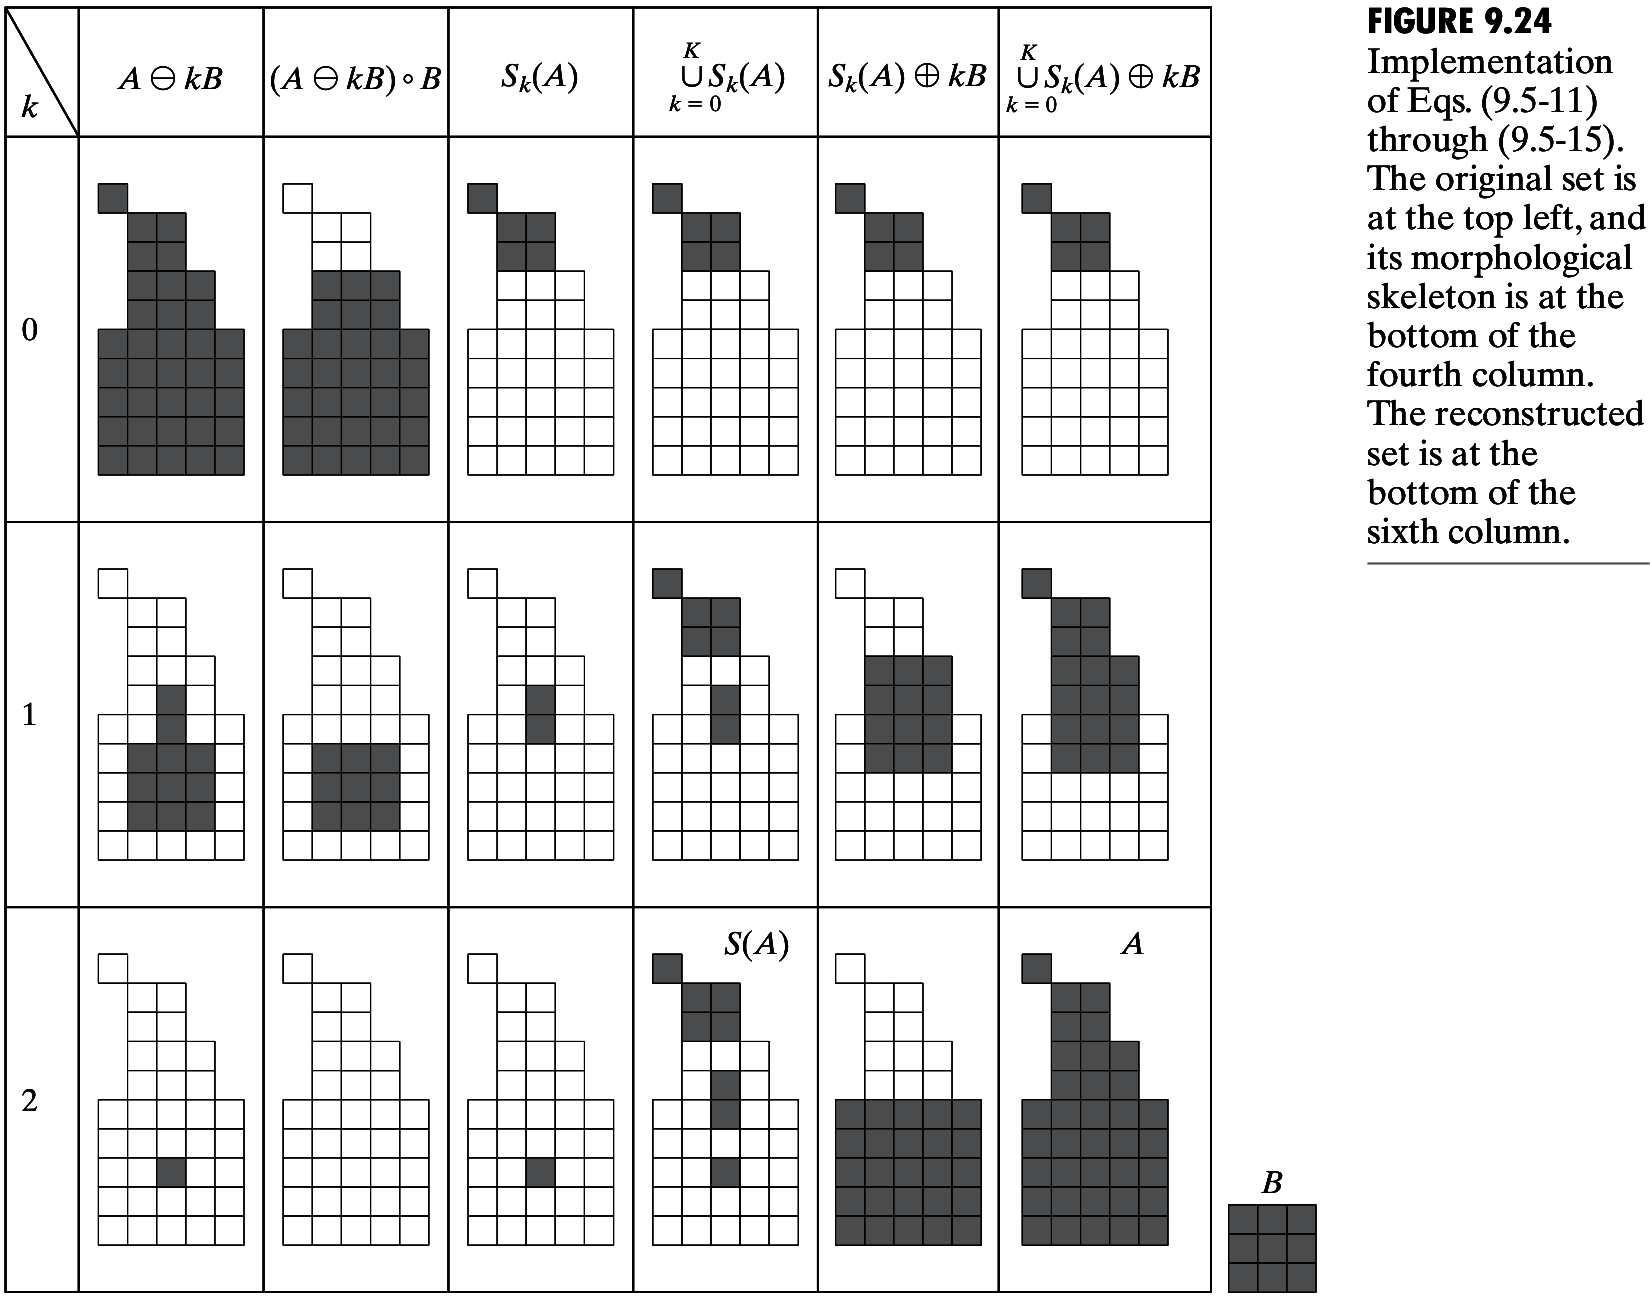
\includegraphics[width=.8\textwidth]{fig-9-24.png}
\end{figure}
\end{frame}

\subsection{Pruning}

\begin{frame}
\frametitle{Pruning}
\begin{columns}
\begin{column}{.5\textwidth}
\begin{itemize}
\item Used for cleaning the result of thinning and skeletons.
\end{itemize}
Algorithm:
\begin{enumerate}
\item Thin $X_{1} = A \otimes B$.
\item Find endpoints $X_{2} = \bigcup_{k=1}^{8} (X_{1} \circledast B^{k} )$.
\item Fill region $X_{3} = (X_{2} \oplus H ) \cap A$, where $H = \texttt{ones}(3)$.
\item Result $X_{4} = X_{1} \cup X_{3}$.
\end{enumerate}
\end{column}
\begin{column}{.5\textwidth}
\begin{figure}[!h]
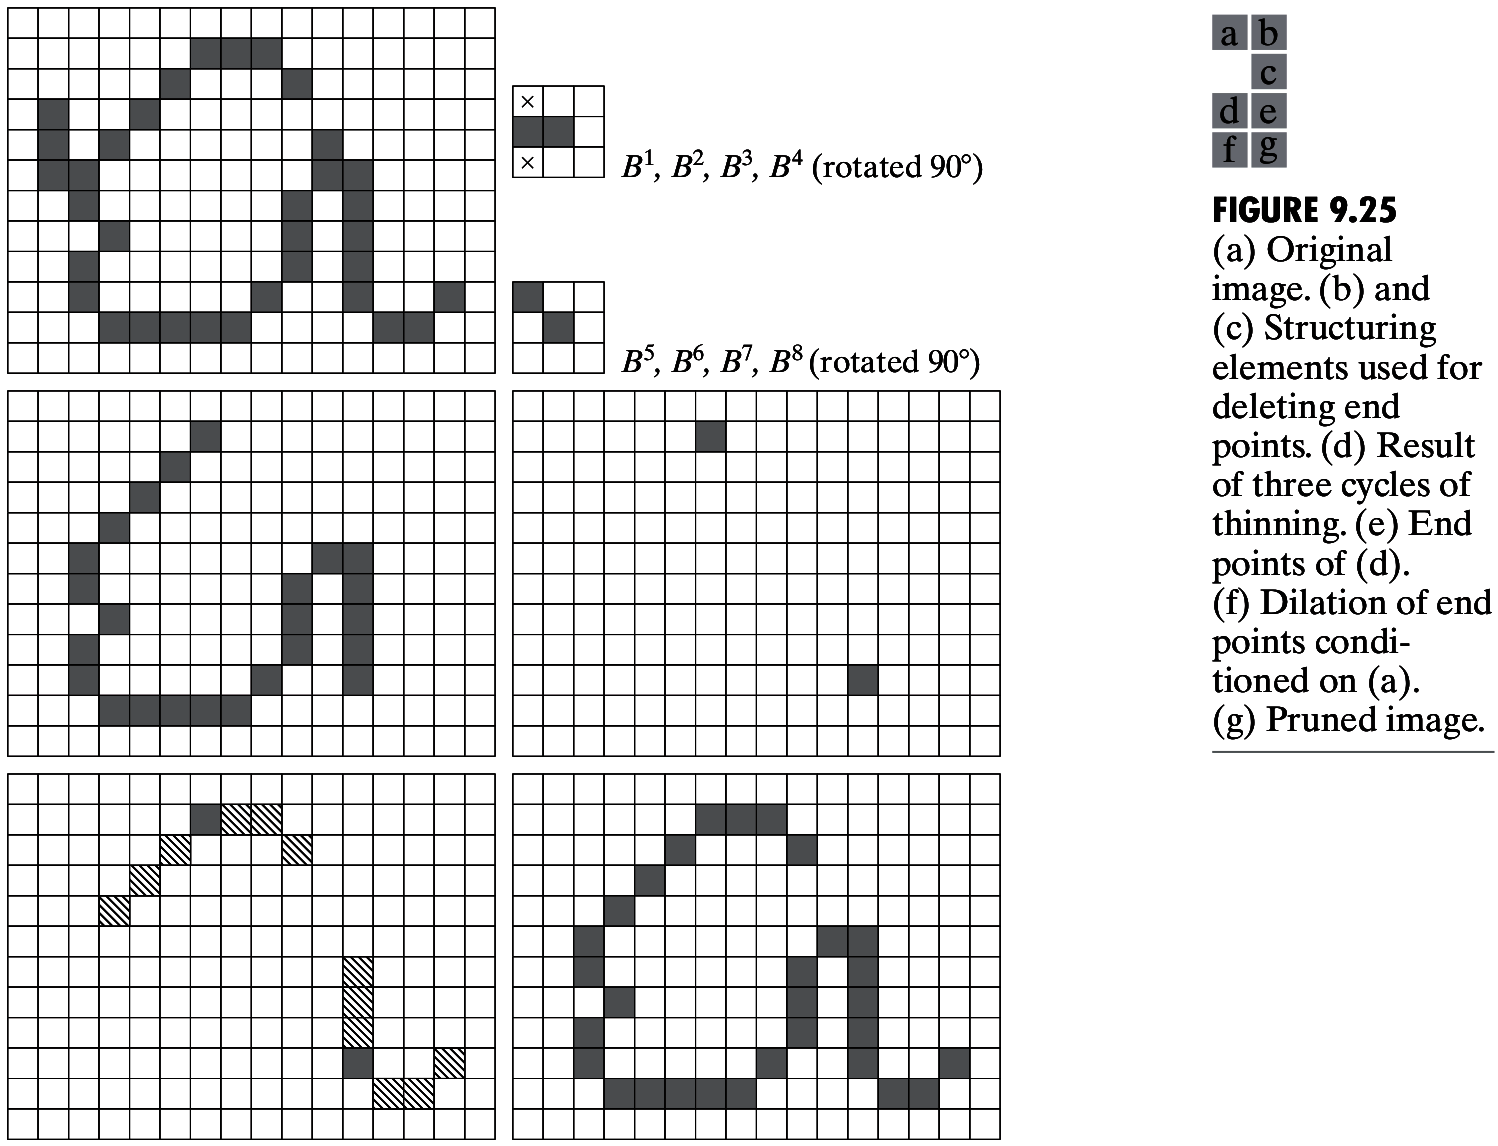
\includegraphics[width=\textwidth]{fig-9-25.png}
\end{figure}
\end{column}
\end{columns}
\end{frame}

\section{Morphological reconstruction}

\begin{frame}
\frametitle{Morphological reconstruction}
Reconstruction is a morphological transformation involving two images and a structuring element:
\begin{enumerate}
\item Marker: Starting point for the transformation.
\item Mask: Constrains the transformation.
\item Structuring element: Defines connectivity.
\end{enumerate}
Matlab: \texttt{imreconstruct(marker, mask)}.
\end{frame}

\begin{frame}
Algorithm ($G$ is the mask):
\begin{enumerate}
\item Initialize $h_{1}$ to be the marker image, $F$ s.t. $F \subseteq G$.
\item Create SE $B$ = \texttt{ones(3)}.
\item Repeat
\[
h_{k+1} = \left ( h_{k} \oplus B \right ) \cap G
\]
until $h_{k+1} = h_{k}$.
\item $R_{G}(F) = h_{k+1}$.
\end{enumerate}
Notice that hole filling $X_{k} = \left ( X_{k-1} \oplus B \right ) \cap A^{c}$ is a particular case of image reconstruction.
\end{frame}

\begin{frame}
\begin{figure}[!h]
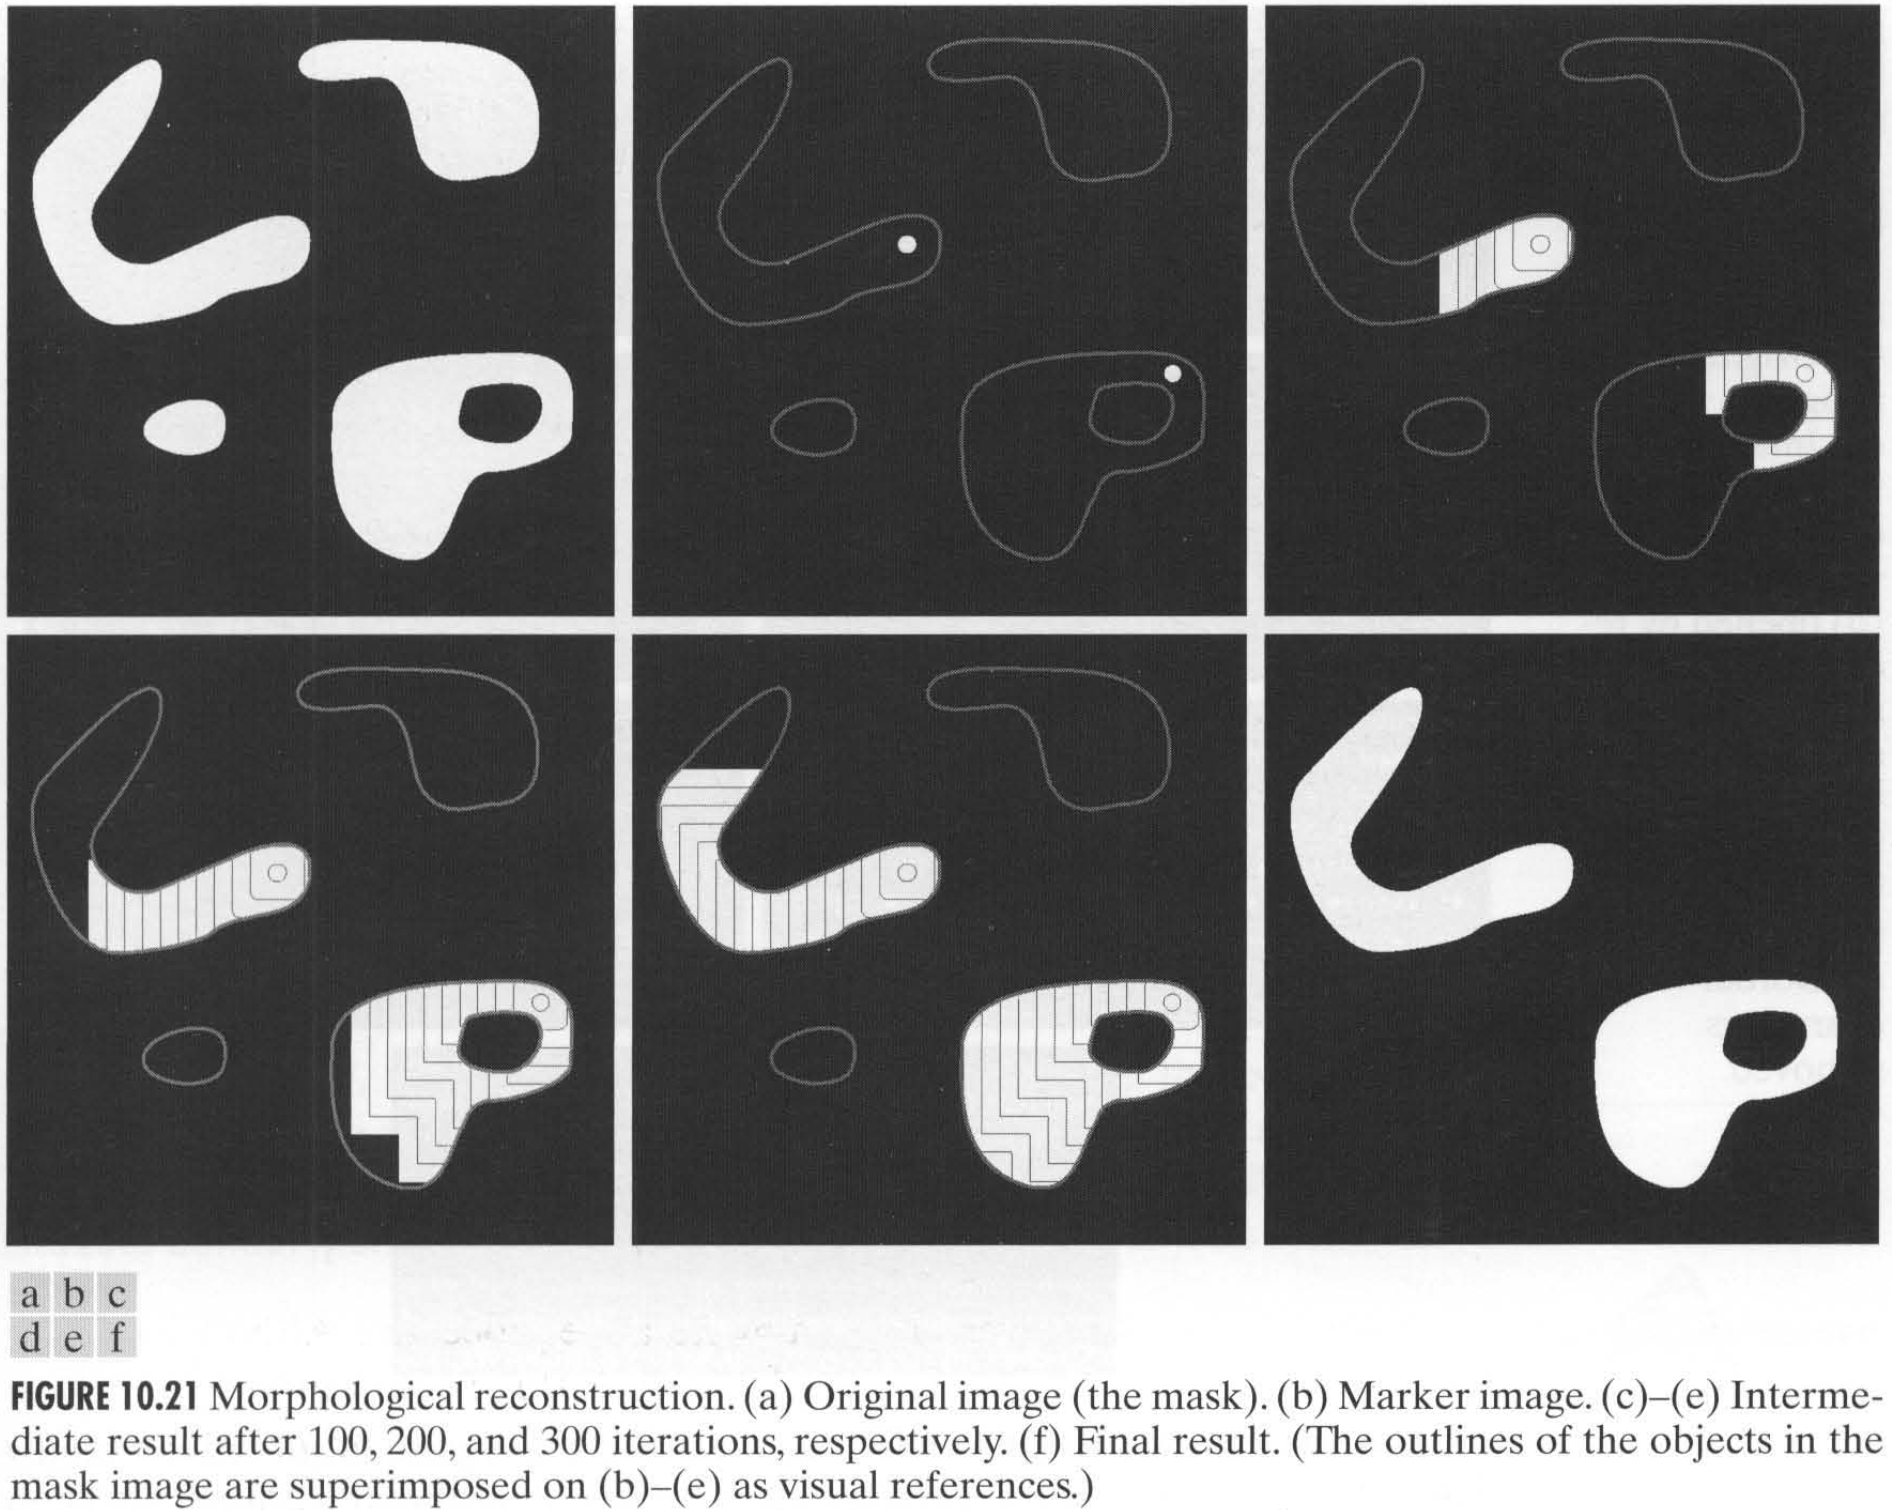
\includegraphics[width=.8\textwidth]{fig-10-21.png}
\end{figure}
\end{frame}

\subsection{Opening by reconstruction}

\begin{frame}
\frametitle{Opening by reconstruction}
Opening:
\begin{enumerate}
\item erosion (removes small objects), followed by a;
\item dilation (restores the shapes of remaining objects, depending on SE shape).
\end{enumerate}
Opening by reconstruction restores the original shapes of the remaining objects.\\
It is defined as:
\[
R_{G} (G \ominus B).
\]
\end{frame}

\begin{frame}
\begin{figure}[!h]
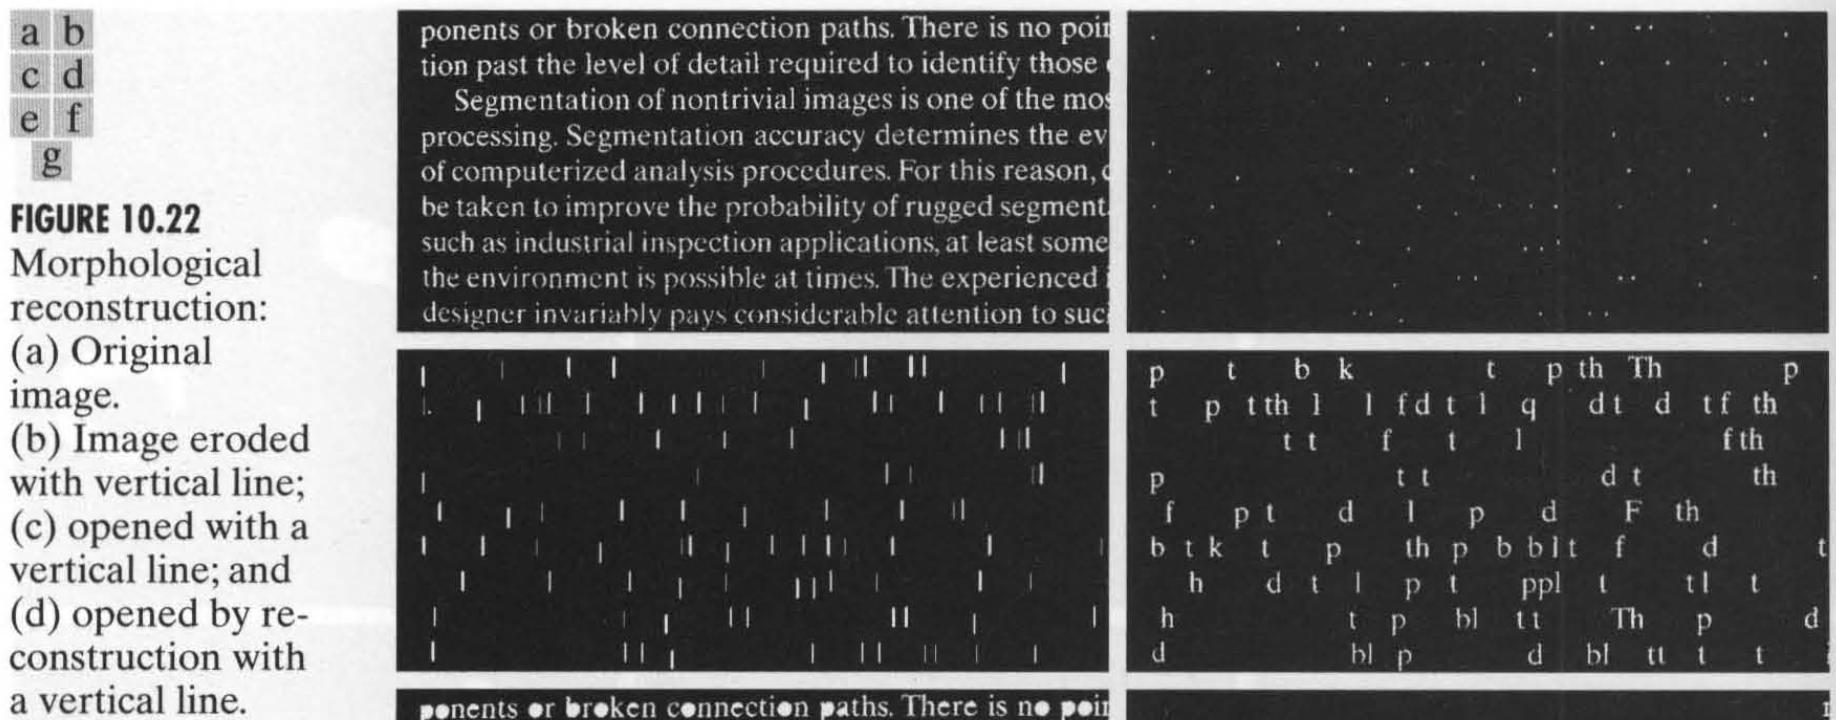
\includegraphics[width=\textwidth]{fig-10-22}
\end{figure}
\end{frame}

\subsection{Filling holes}

\begin{frame}
\frametitle{Filling holes}
Let:
\begin{enumerate}
\item $I(x,y)$ - binary image.
\item Marker image $F$ to be 0 everywhere except on the image border:
\[
F(x,y) = \left \{
\begin{array}{ll}
1 - I(x,y) & \text{if }(x, y)\text{ is on the border of }I\\
0 & \text{otherwise}
\end{array}
\right .
\]
Then
\[
H = \left [ R_{I^{c}}(F) \right ]^{c}
\]
is a binary image equal to $I$ with all holes filled.
\end{enumerate}
Matlab: \texttt{g = imfill(f, 'holes')}.
\end{frame}
%
%\begin{frame}
%\frametitle{Filling holes}
%\begin{figure}[!h]
%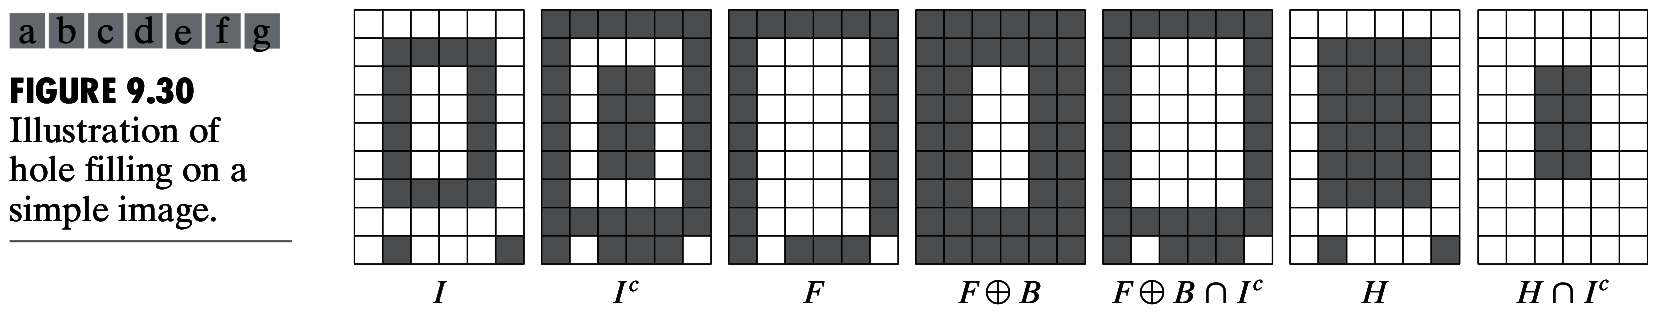
\includegraphics[width=\textwidth]{fig-9-30}
%\end{figure}
%\end{frame}

\begin{frame}
\begin{figure}[!h]
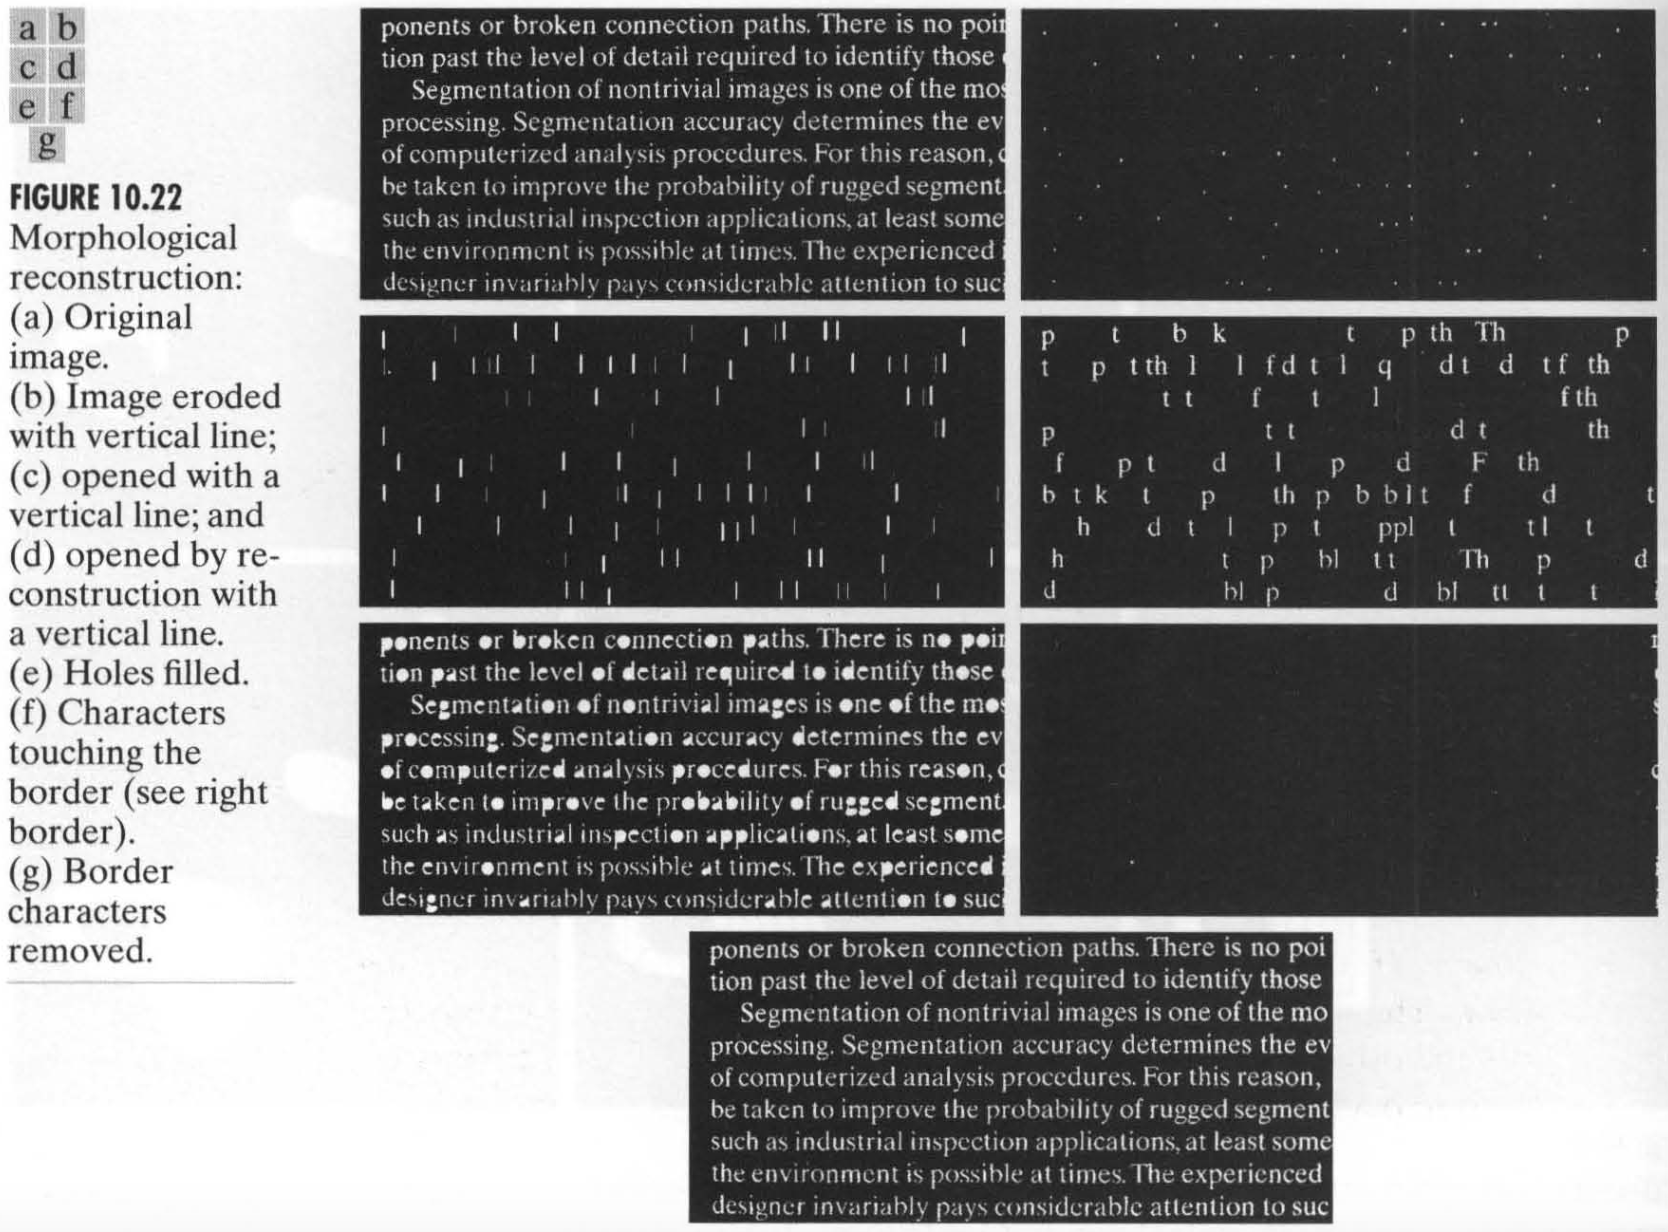
\includegraphics[width=.75\textwidth]{fig-10-22-all}
\end{figure}
\end{frame}

\subsection{Clearing border objects}

\begin{frame}
\frametitle{Clearing border objects}
Remove objects touching the border of the image.\\
Define marker $F$ as
\[
F(x,y) = \left \{
\begin{array}{ll}
I(x,y) & \text{if }(x, .y)\text{ is on the border of }I\\
0 & \text{otherwise}
\end{array}
\right .
\]
Then
\[
H = R_{I}(F)
\]
contains only objects touching the border.\\
Matlab: \texttt{g = imclearborder(f, conn)}.
\end{frame}

\begin{frame}
\begin{figure}[!h]
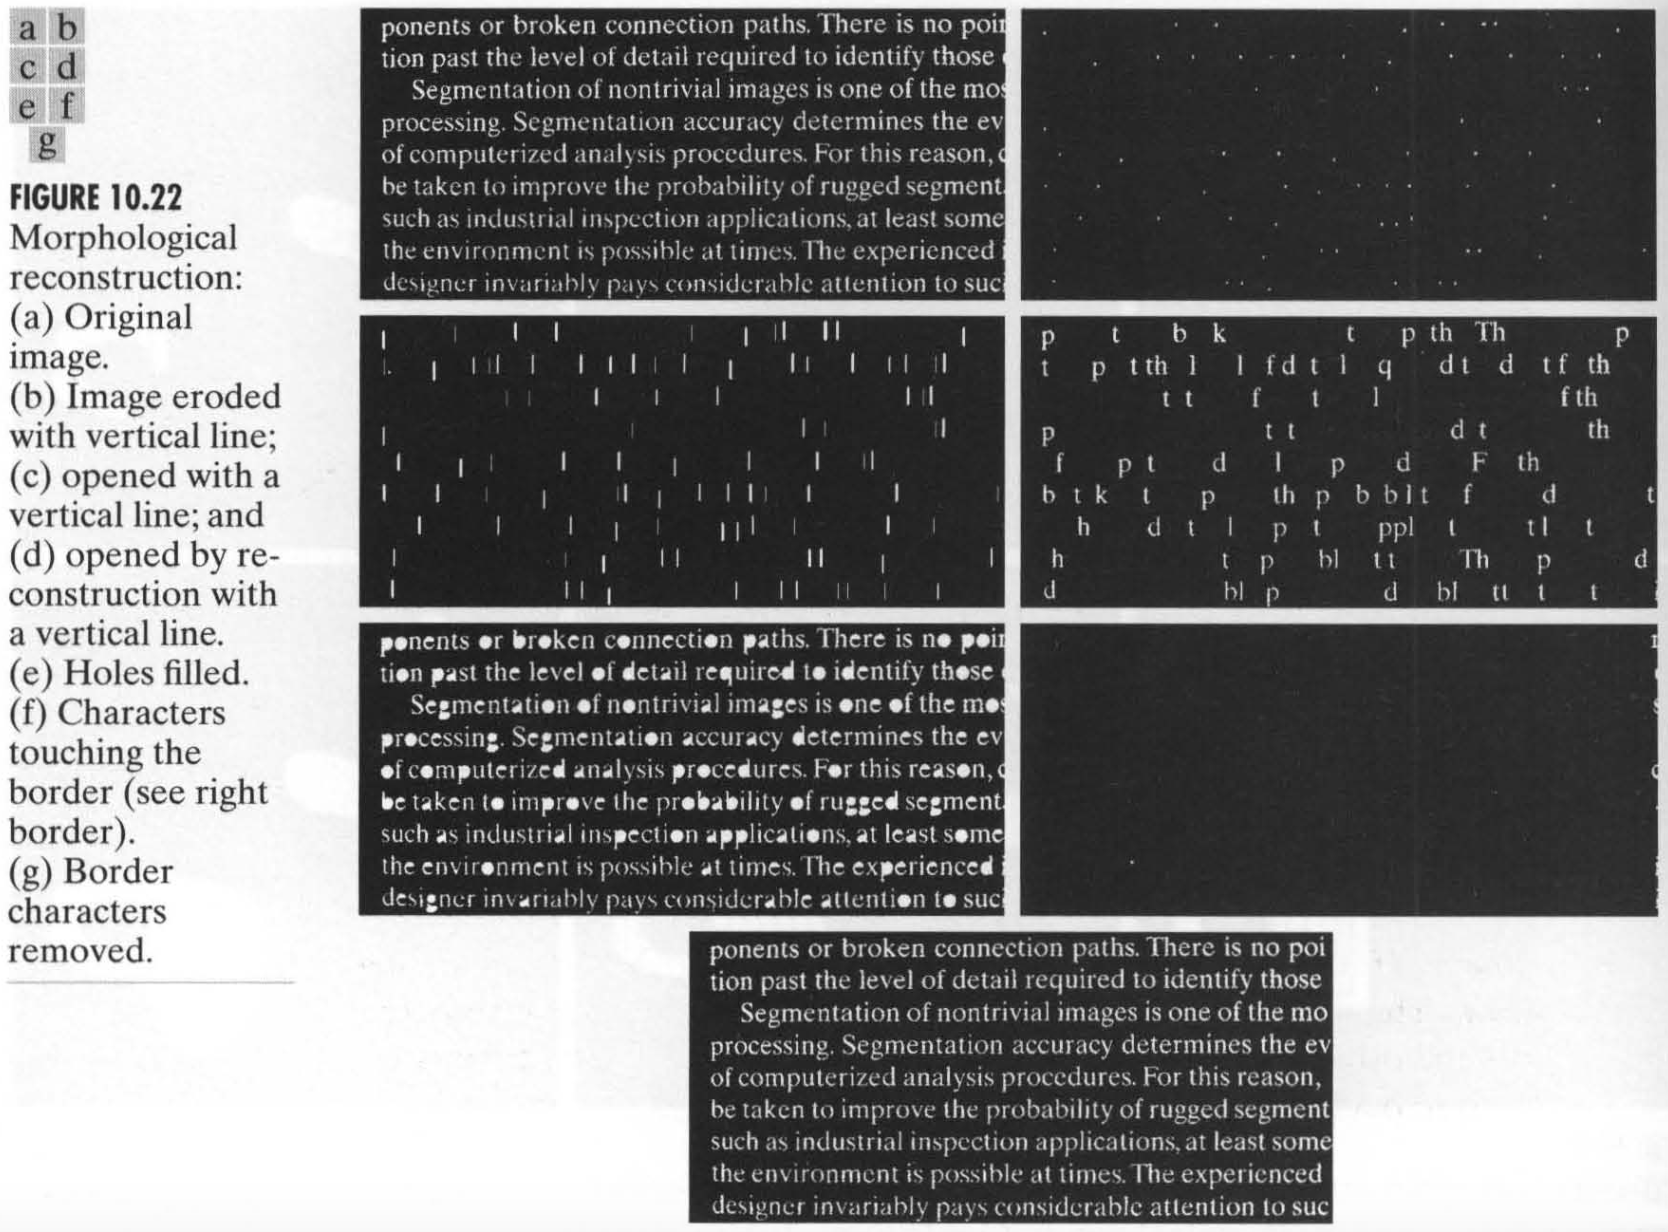
\includegraphics[width=.75\textwidth]{fig-10-22-all}
\end{figure}
\end{frame}

\section{Summary of operators}

\begin{frame}
\frametitle{Summary of operators}
\begin{figure}[!h]
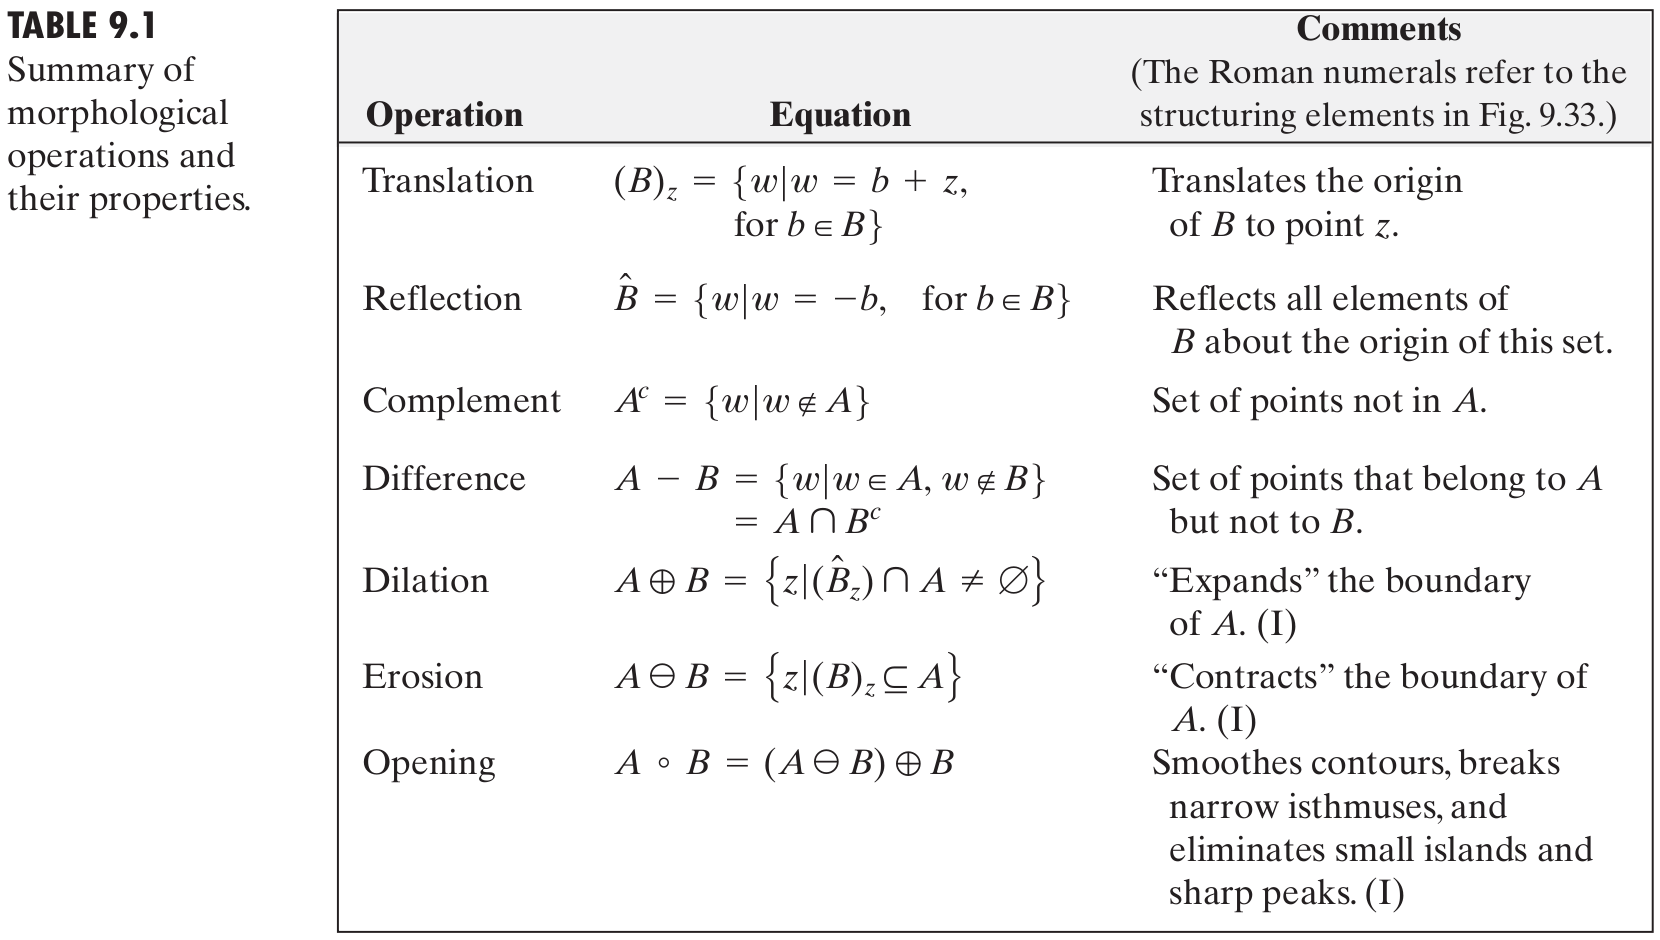
\includegraphics[width=\textwidth]{table-9-1}
\end{figure}
\end{frame}

\begin{frame}
\begin{figure}[!h]
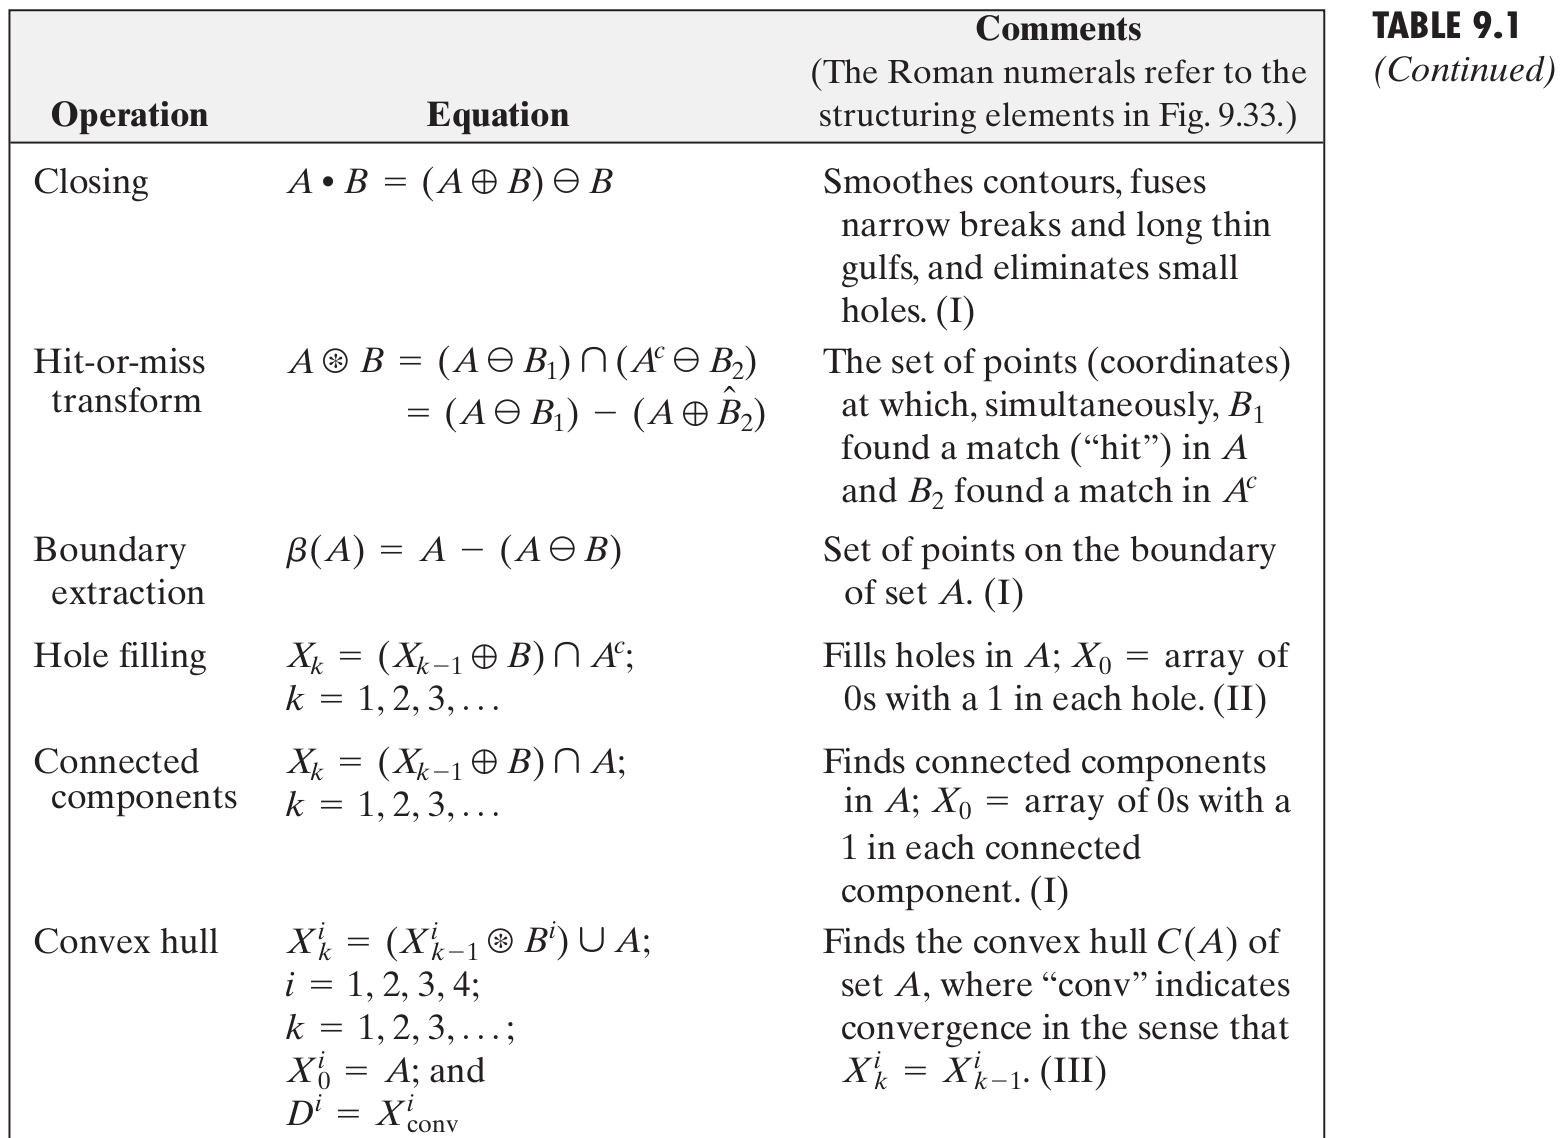
\includegraphics[width=.8\textwidth]{table-9-1-1}
\end{figure}
\end{frame}

\begin{frame}
\begin{figure}[!h]
\includegraphics[width=.8\textwidth]{table-9-1-2}
\end{figure}
\end{frame}

\begin{frame}
\begin{figure}[!h]
\includegraphics[width=.7\textwidth]{table-9-1-3}
\end{figure}
\end{frame}


\begin{frame}
\begin{figure}[!h]
\includegraphics[width=.7\textwidth]{table-9-1-4}
\end{figure}
\end{frame}

\begin{frame}
\begin{figure}[!h]
\includegraphics[width=\textwidth]{fig-9-33}
\end{figure}
\end{frame}

\section{Gray-Scale Morphology}

\begin{frame}
\frametitle{Gray-Scale Morphology}
We now deal with digital functions:
\begin{itemize}
\item $f(x,y)$ - input image.
\item $b(x,y)$ - structuring element (SE).
\end{itemize}
These functions are discrete:
\begin{itemize}
\item $x$ and $y$ are integers.
\item $f$ and $b$ assign an intensity value to each pair $(x,y)$.
\end{itemize}
\end{frame}

\subsection{Gray-scale dilation}

\begin{frame}
\frametitle{Gray-scale dilation}
Definition of gray-scale dilation:
%The dilation of $f$ by a \textit{flat} SE $b$ at $(x,y)$ is the \textit{max val} in the windows delimited by $\hat{b}$ centered at $(x,y)$:
\[
\left [ f \oplus b \right ] \left ( x, y  \right ) = \max_{(s,t)\in b} \left \{ f(x-s, y-t) + b(s,t) \right \}
\]
\begin{figure}[!h]
\includegraphics[width=.5\textwidth]{gs-dilation-ex-1.png}
\end{figure}
\end{frame}

\begin{frame}
\begin{itemize}
\item Similar to convolution.
\item $\max$ operation substitutes convolution sum.
\item Addition substitutes the product in the convolution sum.
\end{itemize}
General effects:
\begin{itemize}
\item For positive values of the SE, the resulting image tends to be brighter.
\item Dark details are reduced or eliminated, depending on how the values and shapes of the details are related to the SE.
\end{itemize}
\end{frame}

\subsection{Gray-scale erosion}

\begin{frame}
\frametitle{Gray-scale erosion}
Definition of gray-scale erosion:
%The \textit{erosion} of $f$ by a \textit{flat} structuring element $b$ at any location $(x,y)$ is defined as the \textit{minimum} value of the image in the region coincident with $b$ when the origin of $b$ is at $(x,y)$:
\[
\left [ f \ominus b \right ] \left ( x, y  \right ) = \min_{(s,t)\in b} \left \{ f(x + s, y + t) - b(s,t) \right \}
\]
\begin{figure}[!h]
\includegraphics[width=\textwidth]{gs-erosion-ex-1.png}
\end{figure}
\end{frame}

\begin{frame}
\begin{itemize}
\item Similar to correlation.
\end{itemize}
General effects:
\begin{itemize}
\item If the SE has positive values, the result tends to be darker.
\item Bright details smaller than the SE are reduced, according to the SE's values and shape.
\end{itemize}
\end{frame}

\begin{frame}
\begin{figure}[!h]
\includegraphics[width=\textwidth]{fig-9-32.png}
\end{figure}
\end{frame}

\subsection{Gray-scale opening}

\begin{frame}
\frametitle{Gray-scale opening}
Defined as
\[
f \circ	b = (f \ominus b) \oplus b.
\]
\begin{figure}[!h]
\includegraphics[width=.7\textwidth]{fig-10-24.png}
\end{figure}
\end{frame}

\subsection{Gray-scale closing}

\begin{frame}
\frametitle{Gray-scale closing}
Defined as
\[
f \bullet b = (f \oplus b ) \ominus b.
\]
\begin{figure}[!h]
\includegraphics[width=.8\textwidth]{fig-10-24-2.png}
\end{figure}
\end{frame}

\subsection{Gray-scale opening and closing}


\begin{frame}
\frametitle{Gray-scale opening and closing}
\begin{figure}[!h]
\includegraphics[width=\textwidth]{fig-9-37.png}
\end{figure}
\end{frame}

\begin{frame}
\begin{itemize}
\item Opening suppresses bright details smaller than the structuring element.
\item Closing suppresses dark details smaller than the structuring element.
\item Both are often combined for smoothing and noise removal.
\end{itemize}
\end{frame}

\begin{frame}
Morphological smoothing:
\begin{itemize}
\item Opening followed by closing, ie., $(f \circ b) \bullet b$.
\item Effect: removal of bright and dark artifacts and noise.
\end{itemize}
\begin{figure}[!h]
\includegraphics[width=.6\textwidth]{fig-9-38.png}
\end{figure}
\end{frame}

\begin{frame}
Morphological gradient:
\begin{itemize}
\item $g = (f\oplus b) - (f \ominus b)$.
\item highlights borders.
\item less dependent of border direction than Sobel.
\end{itemize}
\begin{figure}[!h]
\includegraphics[width=.6\textwidth]{fig-9-39.png}
\end{figure}
\end{frame}

\subsection{Top-hat and bottom-hat transforms}

\begin{frame}
\frametitle{Top-hat and bottom-hat transforms}
\begin{columns}
\begin{column}{.5\textwidth}
Top-hat:
\[
T_{\text{hat}} (f) = f - (f \circ b)
\]
Bottom-hat:
\[
B_{\text{hat}} (f) = (f \bullet b) - f
\]
\end{column}
\begin{column}{.5\textwidth}
Applications:
\begin{itemize}
\item Removing objects by using a SE smaller than the object.
\item Top-hat: light objects on dark background.
\item Bottom-hat: dark objects on bright background.
\end{itemize}
\end{column}
\end{columns}
\end{frame}

\begin{frame}
\frametitle{Gray-scale opening and closing}
\begin{figure}[!h]
\includegraphics[width=.8\textwidth]{fig-9-40.png}
\end{figure}
\end{frame}

\subsection{Granulometry}

\begin{frame}
\frametitle{Granulometry}
\begin{figure}[!h]
\includegraphics[width=\textwidth]{granulometry.png}
\end{figure}
\end{frame}

\subsection{Texture segmentation}

\begin{frame}
\frametitle{Texture segmentation}
\begin{figure}[!h]
\includegraphics[width=.5\textwidth]{textureSegmentation.png}
\end{figure}
\end{frame}

\subsection{Gray-scale morphological reconstruction}

\begin{frame}
\begin{figure}[!h]
\includegraphics[width=.6\textwidth]{gs-reconstruction.png}
\end{figure}
\end{frame}

%%--------------------------------
%-- REFERENCES
%\begin{frame}
%References:
%\begin{itemize}
%\item \href{http://homepages.inf.ed.ac.uk/rbf/HIPR2/open.htm}{http://homepages.inf.ed.ac.uk/rbf/HIPR2/open.htm}
%\end{itemize}
%\end{frame}

\end{document}